
\documentclass[letterpaper,13pt,single,pdftex]{scrartcl}
%\usepackage[ngerman]{babel}
\usepackage{color}
\usepackage{amsmath}
\usepackage{times}
\usepackage{graphicx}
\usepackage{fancyheadings}
\usepackage{enumitem}
\setlist[enumerate]{label*=\arabic*.}
\usepackage{hyperref}
\usepackage{amstext}
\setlength{\parindent}{0.6pt}
\setlength{\parskip}{0.6pt}
\usepackage{scalerel,amssymb}
\def\msquare{\mathord{\scalerel*{\Box}{gX}}}
\usepackage[letterpaper,  margin=1in]{geometry}
\newenvironment{rcases}
  {\left.\begin{aligned}}
  {\end{aligned}\right\rbrace}
\title{ECON 601 Lecture Notes}
\author{Yanan Hou}
\renewcommand{\baselinestretch}{1.5}
 

\begin{document} 


\section{ Consumer Theory}
\subsection{Primitive notions}
\subsubsection{consumption set/choice set X}
$\bullet$ \textbf{Properties/assumptions}
\begin{enumerate}
    \item 
    $\O \ne x \subseteq R^n_+$
    \item
X is close
\item
X is convex
\item
$O \in X$
\end{enumerate}

$\bullet$ \textbf{Definition of set}\\
a set is closed it if includes all limit points or boundaries\\
a set is open if its complement is closed \\
A = [0,1]  closed  \quad B=(0,1] neither \quad C=(0,1)open\\
set can be convex or non-convex \text{Unless stated otherwise} \quad $X = R^n_+$
\subsubsection{Consumption Bundle}
 \[ \textbf{x} = (x_1,\dots,x_n) \in \textbf{X} \subseteq R^n_+ \]
 $x_i =$ \text{amount of good i,}\quad  $x_i \in R_+\,, x_i \ge  0$
\subsection{Preferences and Utility}
\subsubsection{Preferences Relations}
 $ \textbf{x}^1 = (x^1_1,x^1_2,x^1_3,\dots,x^1_n)$ \\$\textbf{x}^2 = (x^2_1,x^2_2,x^2_3,\dots,x^2_n)$
\par \textbf{Definition}\\
 $x^1 \succeq x^2 $ 
 ($x^1$ is at least as good as $x^2$)

\par \textbf{Strict Preference Relation}\\
 $x^1 \succ x^2  \Leftrightarrow  x^1 \succeq x^2\, and\, x^2 \not\succeq x^1$

\par \textbf{Indifference}\\
 $x^1 \sim x^2 \Leftrightarrow x^1 \succeq x^2 \text{, and } x^2 \succeq x^1$\\

$\bullet$\textbf{Axioms of Consumer choice}

    \textbf{Axiom 1 Completeness}\\
 For all $x^1, x^2 \in X, x^1 \succeq x^2 \,or \,x^2 \succeq x^1$, or \,both\\
Rule out I don't know

 \textbf{Axiom 2 Transitivity}
 \\ Let $x^1 ,x^2$ and $x^3 \in X$, if $x^1 \succeq x^2, \& x^2 \succeq x^3$, then $x^1 \succeq x^3$




\textbf{Axiom 1 \& 2 $\Rightarrow$ the consumer can rank all the bundle from best to worst}\\

\text{Problem: Because $X = R^n_+$ is uncountable, Axiom $1\& 2\not\Rightarrow u(x)$\\}

 \textbf{Axiom 3 Continuity}
 \\$ B(x) =  \{y\in X | y \succeq x\}  \leftarrow $ better than set\\
 $W(x) = \{y\in X|x \succeq y\} \leftarrow$ worse than set\\
 $B(x)$ and $W(x)$ are closed in $R^n_+$
\\Suppose $y^k$ is a sequence of bundles, such that $y^k\in B(x)$ i.e
\[y^k \succeq x, \forall k\]
If $y^k \rightarrow y$ (as $k\rightarrow\infty$), then $ y\in B(x) \,i.e, \,y\succeq x$\\

E.g. Lexicographic preference: uncountable X\\
$x^1 = (x_1^1, x_2^1) \quad x^2 = (x_1^2, x_2^2)$\\
(2,0) $\succ$ (1,5)\\
(1,0) $\nsucc$ (1,5)\\
Complete transitive but not continuous. \\
$y^k=(\frac{1}{k},0)$\\
$x=(0,1)$\\
$y^k \succ x,\,\forall \,k$\\
$y^k \rightarrow (0,0) \nsucc (0,1)$\\
B(x) is not closed(not continuous)\\

Completeness $+$ Transitivity $\Rightarrow$ Rational preferences $\Rightarrow$ X are countable + $u(x)$ - utility function\\



\par \textbf{Axiom 4' Local Non-satiation}
\\$\succeq$ is locally non-satiation if $\forall x\in X $ and $\forall \varepsilon > 0$, there is $x'$ such that $d(x,x') < \varepsilon$ and $x'>x$ (d means distance)\\

\par \textbf{Axiom 4 Monotonicity}
 \\\text{Weak: If $x^1 \ge x^2$, then $x^1 \succeq x^2 $ \,$[ x^1 \succeq x^2 \Leftrightarrow \,x^1_i \ge x^2_i,\,\forall i]$}

 \text{Strict: If $x^1 > x^2$, then $x^1 \succ x^2$ [$x^1 \succ x^2 \Leftrightarrow \, x^1_i > x^2_i, \forall i]$}

 \text{Strong: If $x^1\ge x^2 $ and $x^1 \ne x^2, x^1 \succ x^2$}

 \text{Claim: If $\succeq$ is complete, transitive, continuous and monotonic, then it has a utility function}\\
 \underline{Proof}:
 Take $x\in X = R^n_+$, by monotonicity\\
 $(max_i \,x_i, \dots, max_i\, x_i)\succeq x \succeq(0, \dots, 0) $\\
 By continuity, there is a unique bundle. 
\begin{align*}
    (t(x), \dots,t(x)) \sim x &\text{   set }u(x) = t(x)\\
    x\succeq y \Leftrightarrow &(t(x), \dots, t(x)) \succeq (t(y),\dots,t(y))\\
    \Leftrightarrow & t(x)\ge t(y)\\
    \Leftrightarrow & u(x)\ge u(y)
\end{align*} 

$\succeq$ completeness, transitivity, continuity $\Rightarrow\, \exists $ a continuous u(x) \\
Monotonicity $\Rightarrow$ "More is better" $\Rightarrow$ increasing u(x)\\
A utility function exists if 
\begin{enumerate}
    \item complete +transitive + finite X
    \item complete +transitive + countable (can be infinite)
    \item complete +transitive + continuous 
\end{enumerate}
\textbf{Axiom 5 Convexity}
 \[x^1 \succeq x^2 \Rightarrow \alpha x^1+(1-\alpha)x^2 \ge x^2, \forall \alpha \in [0,1]\]
\textbf{Strict convexity}
 \[ x^1 \succeq x^2 \text{and } x^2 \ne x^1 \Rightarrow \alpha x^1+(1-\alpha)x^2 > x^2, \forall \alpha \in (0,1)\]
Roughly, convexity means that individual dislikes extremes.\\

\begin{rcases}
    u(x^1) \ge u(x^2) \Rightarrow u(\alpha x^1 + (1-\alpha) x^2)\ge u(x^2)\\  \Leftrightarrow u(\alpha x^1 +(1-\alpha)x^2) \ge min\{u(x^1), u(x^2)\}
\end{rcases}

 $\Leftrightarrow$ u is quasi-concave\\
 
u is q-concave iff ($\iff$) \{$x\in R^n_+| u(X) \ge u_1$\} is convex for all $u_1$, where \{$x\in R^n_+| u(X) \ge u_1$\} is "Better than set"("Upper Contour)


 u(x) is strictly quasi-concave iff MRS is strictly decreasing

\par \textbf{Concave u(x)}
 \[ u(\alpha x^1 +(1-\alpha)x^2 ) \ge \alpha x^1 + (1-\alpha) x^2  {\ge min\{u(x^1), u(x^2)\} } \]
concave u(x) $\Rightarrow$ quasi-concave u(x)\\
u is quasi-concave $\Rightarrow$ r=f(u) is also q-concave (f is strictly increasing)\\
$f(x) = x^{\frac{1}{2}}, x\in R_+, \rightarrow $ concave\\
$(f(x))^4 \Rightarrow$ convex\\
In non-linear utility, convex has no flat part indifferent curve\\
\includegraphics[scale=0.4]{graph/consumer-01.jpg}

\subsubsection{The Utility Function}
 \text{Suppose X is finite, $x^1 \succeq x^2 \succeq  \dots \succeq x^k, \\ u(x^1) = k, u(x^2) = k-1, \dots, u(x^k) = \leftarrow$ utility function\\}
 Suppose X is countable(can be infinite) $\rightarrow$ Utility function\\
$\bullet$ \textbf{Definition}: \\
A real-valued function u:$X\rightarrow \,R$ such that $ x\succeq y \Leftrightarrow u(x) \ge u(y)$\\
$X = R^n_+ = R_+ \times\dots\times R_+$\\
$x = (x_1,\dots, x_n)$ mark\\
$\bullet$ \textbf{Debreu Theorem}\\
If $\succeq$ is complete, transitive continuous, then there is a continuous $u(X)$ that represents $\succeq$}\\
Conversely, if a continuous u(X) represent $\succeq$, then $\succeq$ is continuous.\\
$\bullet$\textbf{Transitivity:  }
\[ u(x) \ge u(y) \ge u(z) \Leftrightarrow x \succeq y \succeq z\]
Lexicographic preference have no utility representation\\
Proof:  suppose they do, then for any $x_i \in R_+$
\[(x,1) \succ (x,0) \text{[Lexicographic]}\]
\[\Leftrightarrowightarrow u(x,1) >u(x,0)\]
\underline{Fact: Rational numbers are dense in real life.}\\
Then, there 's a rational number $q(x_1)$ such that $u(x,1) >q(x_1) > u(x,0)$\\
\underline{Fact: Rational numbers are countable.}\\
Claim: $q(x_1):\, R_+ \, \rightarrow $ Rationals is one-to-one.\\
Proof: Take $x_1 \succ x_1'$, then $q(x_1)>u(x,0)>u(x_1',1) \Rightarrow q(x_1)>q(x_1')$\\
$\Rightarrow$ q is a function strictly increasing in x, and thus a one-to-one mapping.\\
But q maps real numbers into rationals and therefore, implies that real numbers are countable, a contradiction. Hence, there is $u(x)$ for lexicographic preference. \\

$\bullet$\textbf{Theorem: Non-uniqueness of utility}
 \\If u(x) represents $\succeq$, then for every strictly increasing function f: $R \rightarrow R$, the function $V(x) = f(u(x))$ also represents $\succeq$\\
\underline{Proof}:
\begin{align*}
    \begin{rcases}
     x\succeq y &\Rightarrow u(x) \ge u(y)\\
    &\Rightarrow f(u(x)) \ge f(u(y))\\
    &\Rightarrow v(x) \ge v(y)
    \end{rcases}
   x\succeq y \Rightarrow v(x) \ge v(y)
\end{align*}
$u(x_1,x_2) = x_1^{\frac{1}{2}} x_2^{\frac{1}{2}}$\\
$v(x_1,x_2)= (x_1^{\frac{1}{2}} x_2^{\frac{1}{2}})^2 = x_1 x_2$

\subsection{The Consumer's problem}
Let $p = (p_1,p_2, \dots,p_n) \in R^n_{++},\, p_i>0$\\
$I\ge 0$, fixed income
\begin{align*}
    max_x \quad &u(x)\\
    s.to \quad &px\le I [\sum\limits_{i=1}^{n}p_ix_i \le I]\\
    &x\ge 0
\end{align*}
Continuity,completeness, transitivity $\Rightarrow$ Continuous u(x)
\subsubsection{\latex Budget set\\$ B = {\{x \in R^n_+ | \textbf{px} \le I\ \}}$}
\par \textbf{compact}
\left\{
\begin{array}{ll}
    &\text{bounded}: $x_i \le I/p_i$\\
    &\text{closed}: $x^k = (x^k_1, x^k_2, \dots,x^k_n)$, suppose $x^k \rightarrow x$ 
\end{array}
\right\\

 $B \ne \O$ because $O \in B$ if $px^k \le I$, then $px\le I\Leftarrow $ closed. \\(If take the convergence in the set, limit is in the set $\Rightarrow$ closed)\\
 \forall \varepsilon >0, \exists $k_o,\quad s.t \quad d(x,x^k)<\varepsilon, \forall k \ge k_0$\\
 \includegraphics[scale = 0.2]{graph/consumer-02.jpg}\\
Continuous u(x) and non-empty compact B $\Rightarrow$ there is a solution to consumer problem

\subsubsection{Utility-maximization problem}
\par \textbf{Marshallian Demand(Ordinary demand)}
 \\Let $ x^* = x(p.I)$ be a solution \\ $x^*$ is unique if utility is strictly quasi-concave( budget set is compact and convex) or $\succeq$ is strictly convex\\
\includegraphics[scale=0.3]{graph/consumer-03.jpg}\\
 $ max\limits_{x}\quad u(x) \quad\quad $ s.t. $ \textbf{p.x} \le \textbf{I}$
 \\FOC: $f'(x) = 0 \Rightarrow x^*$\\SOC: $f''(x) \le 0$

\par \textbf{First order conditions(necessary)}\\
\underline{Kuhn-Tucker Conditions}\\
 $\frac{\partial L}{\partial x_i} = \frac{\partial u}{\partial x_i} - \lambda p_i \le 0$\\$ \frac{\partial L}{\partial x_i}x_i = 0$(Complementary slackness)\\ $i=1,2,\dots,n$\\ $\frac{\partial L}{\partial \lambda}= I -p_0x \ge 0$\\ $\frac{\partial L}{\partial \lambda}.\lambda = 0$, $x \ge 0, \lambda \ge 0$ \\ Suppose $ \frac{\partial u}{\partial x_i} > 0 $ for some i,\\ $\frac{\partial u}{\partial x_i} -\lambda p_i \le 0 \Rightarrow \lambda >0 \Rightarrow \frac{\partial L}{\partial \lambda} = 0, I-px=0$
 \\
 \\ Suppose $x_i^*,x_j^* >0$ \\ 
 \begin{rcases}
     \frac{\partial u}{\partial x_i} - \lambda p_i = 0\\
     \frac{\partial u}{\partial x_j}-\lambda p_j = 0
 \end{rcases}
 $\frac{\partial u/\partial x_i }{\partial u /\partial x_j}=\frac{p_i}{p_j} \Rightarrow$ Marginal rate of substitution \\

\par \textbf{Marginal Rate of Substitution(MRS)}
 \[MRS_{i,j} = -\frac{dx_i}{dx_j}|_{u^0} = \frac{\partial u/ \partial x_i}{\partial u/\partial x_i}\left| _{u^0} \right.}\]
 It is possible that $ MRS_{i,j} \ge \frac{p_i}{p_j}$ (Corner solution)
 \includegraphics[scale = 0.25]{graph/consumer-06.jpg}\\
\left\{
\begin{array}{ll}
      & MRS_{j,i} = 2/1 = \frac{dx_i}{dx_j}, \text{   i is more valuable for this consumer} \\
      & p_i/p_j=1/2, x^*_j = 0 \text{   j is more valuable for others in the market}\\
\end{array}
.\right\\

\textbf{Well-known utility functions}\\
Linear utility [perfect substitution] : $u(x_1,x_2,\dots,\x_n) = \sum{a_ix_i} \,MRS_{i,j} = constant$
\includegraphics[scale=0.3]{graph/consumer-08.jpg}
 \\Cobb-Douglas
 :  $u(x_1,x_2,\dots,x_n = x_1^{a_1} x_2^{a_2}\dots x_n^{a_n}\, \sum{a_ix_i} = 1$ ,$ u(x_1,x_2) = x^{0.5}_1x^{0.5}_2 = u_0$, $x_2 = \frac{u_0^2}{x_1}$
\includegraphics[scale=0.3]{graph/consumer-09.jpg}
 \\Leontief Utility [perfect complement] : $u(x_1,x_2,\dots,x_n) = min \{x_1,\dots,x_n\}\, u_0 = min\{x_1,x_2\}$
\includegraphics[scale = 0.3]{graph/consumer-10.jpg}

\subsection{Indirect Utility and Expenditure}
\subsubsection{The Indirect Utility Function}
\begin{align*}
    v(p,I) = max\, &u(x) &  &v(p,I) = u(x^*(p,I)) \text{maximized utility}\\
    \uparrow \quad s.to \quad & px\le I \quad &\uparrow\\
    \text{indirect utility} \Downarrow \quad &x\ge 0 & &\text{indirect utility}\\
    x^*(p,I)&
\end{align*}
\includegraphics[scale = 0.3]{graph/consumer-11.jpg}\\
$\bullet$\textbf{Properties}\\
If u(x) is continuous and strictly increasing, then 
\begin{enumerate}
    \item 
    v(p,I) is weakly decreasing in $p_i$ and weakly increasing in I\\
    \\
    \fbox{%
    \begin{minipage}{6 in}
    Aside: \\
    \textbf{Envelope theorem}
    \begin{align*}
        max_x\quad &f(x,a) & M(a)=& max_{x,\lambda} \quad L(x,\lambda_1,\dots, \lambda_k)\\
        s.to \quad &g(x,a)\ge 0 & &=f(x,a) +\lambda_1g_1(x,a) +\dots+\lambda_k(x,a)\\
        &\vdots & &\downarrow\\
        &g_k(x,a)\ge0 & &x^*(a),\lambda^*(a)\\
        &x\ge0 & &(x_1^*(a), \dots,x_k^*(a)),(\lambda_1^*(a),\dots,\lambda_k^*(a))\\
        &\Downarrow & &M(a)= L(x^*(a),\lambda^*(a),\lambda)\\
        &&&M'(a) = \sum_i\frac{\partial L}{\partial x_i} . \frac{\partial x_i^*}{\partial a} +\sum_j \frac{\partial L}{\partial \lambda_j}.\frac{\partial \lambda_j^*}{\partial a} +\frac{\partial L}{\partial a}\\
        &&& \qquad \qquad\qquad  0  \qquad \qquad \qquad  0\\
        &&&=\frac{\partial L}{\partial a}(x^*(a),\lambda^*(a),a) -\text{Envelope Thm}
     \end{align*}
    \end{minipage}}\\
    \item
\textbf{Roy's\,Identity}
\[v(p,I) = max _{x,\lambda} L = u(x) +\lambda[I-p_0 x]\]
\[ \frac{\partial v}{\partial p_i} = -\lambda^* x_i^*, \quad \frac{\partial v}{\partial I} = \lambda^* \]
 \[x_i* = - \frac{\partial v/\partial p_i}{\partial v/\partial I} \]
 
    \item
 $v(tp,tI) = v(p,I)$ \\ 
 $t>0 \quad | \quad x*(tp,tI) = x*(p,I) $ \\
 $\Rightarrow v(p,I)$ is homogeneous of degree 0 in $(p,I)$\\
 
 \fbox{%
 \begin{minipage}{6 in}
 Aside: Homogeneous functions\\
 Def: \\
 Let $k \in R$, f(x) is homogenous of degree k (HDK)\\
 if $f(tx) = t^kf(x), f'(x) = HD(K-1)$\\
 $(tx_1, \dots,tx_n), \forall t \in R_{++}$ (Strictly positive)\\
 
 Example:\\
 $f(x) = x^k, x \in R$\\
 $f'(x) = kx^{k-1}$\\
 $f(tx) = t^kx^k = t^kf(x)$
 \end{minipage}}\\
 
 \textbf{Euler's equation}
 \[\text{f(x) is HDK if and only if } \sum\limits_{i=1}^{n}\frac{\partial f(x)}{\partial xi_i} x_i = kf(x) \]
 \[\text{Euler's Equation: } \sum\limits_{i}\frac{\partial v}{\partial p_i}p_i +\frac{\partial v}{\partial I}I = 0\]
    \item
    $v(p,I)$ is quasi-convex in $(p,I)$ \\
    Then $v(p,I)$ is quasi-convex in p.\\
    (A function can be convex in $x_1$ alone, convex in $x_2$ alone,but not convex jointly.)\\
    \textbf{Quasi-convex}: $f(ax' +(1-a)x'')\le max\{f(x'),f(x'')\}$\\
    Average is the worse-than set $\Leftrightarrow$ individual will be worse off at the average of 2. 
    \includegraphics[scale=0.3]{graph/quasi-convex.jpg}\\
    \underline{Proof of property 4}\\
    \fbox{%
    \begin{minipage}{6 in}
    Aside: f(x) is quasi-convex if $f(ax' +(1-a)x'') \le max \{f(x'), f(x'')\}$
    \end{minipage}}\\
    Take$ (P',I')$ and $(P'',I'')$, let $(p^{\alpha}, I^{\alpha})=(\alpha p' +(1-\alpha)p'',\alpha I'+(1-\alpha)I''), \alpha \in [0,1]$\\
    WTS: $V(p^{\alpha}, I^{\alpha}) \le max \{v(p',I'),v(p'',I'')\}$\\
    Suppose $\exists x$ s.t. $p^{\alpha}x \le I^{\alpha}$, but $p'x> I'$ and $p''x>I''$( x is not affordable under $p',p''$)\\
    $\alpha p'x> \alpha I'$ , $(1-\alpha)p''x>(1-\alpha)I''$\\
    Adding side by side, $\alpha p'x +(1-\alpha)p''x> \alpha I'+ (1-\alpha)I''$\\
    $p^{\alpha}x> I^{\alpha}$, a contradiction.\\
    Hence, $p'x \le I'$ or $p''x\le I'', \forall x$ s.t. $p^{\alpha}x \le I^{\alpha}$\\
    $\Rightarrow v(p^{\alpha}, I^{\alpha}) \le v(P',I') or v(P'',I'') \le v(P'',I'')$\\
    $\Rightarrow V(p^{\alpha}, I^{\alpha}) \le max \{v(p',I'),v(p'',I'')\}$
\end{enumerate}
\subsubsection{Constant elasticity of substitution (CES)}
$u(x) = [\sum\limits_{i} (\alpha_i x_i^\varrho)]^{\frac{1}{\varrho}}, \alpha_i \ge 0, \sum\limits_i \alpha_i=1, \varrho\in (-\infty,1)$\\

$\varrho \rightarrow 1 \Rightarrow $Linear utility\\
$\varrho \rightarrow \infty \Rightarrow $ Leontief\\
$\varrho \rightarrow 0 \Rightarrow $ Cobb-douglas\\
$\varrho \rightarrow -\infty \Rightarrow  max\{x_1,x_2\}$\\
$x\in R$, any monotonic function is quasi-concave. \\

\begin{rcases}
     & \text{Strictly quasi-concave} (\varrho <1) \\
     & \text{HD1 in x}
\end{rcases}
$\Rightarrow $ Strictly concave in x\\

$u(x_1, x_2)  = x_1^2x_2^3 = (x_1^{\frac{2}{5}}x_2^{\frac{3}{5})^5$ Not concave since $x_1^2 x_2^3$ each has to be concave but it is quasi-concave with positive monotonic transformation.
\[MRS_{2,1}|_{u_0}=|\frac{dx_2}{dx_1}|_{u_0}\]
Diminishing MRS: $\frac{d MRS_{2,1}}{dx_1}\le 0$\\
\underline{Result}: u(x) is (strictly) quasi-concave if and only if MRS is (strictly) decreasing.\\
Example: \\
$u(x_1,x_2)=x_1x_2 = (x_1^{\frac{1}{2}}x_2^{\frac{1}{2}})$(C-D)\\
$x_1x_2 = u_0 \Rightarrow x_2 = \frac{u_0}{x_1}, MRS_{2,1} = -\frac{dx_2}{dx_1}=\frac{u_0}{x_1^2}$, clearly MRS $\downarrow $ in $x_1$.\\
Wrong way: $MRS_{2,1}|_{u_0} = \frac{\partial u/\partial x_1}{\partial u/\partial x_2} = \underline{\frac{x_2}{x_1}|_{u_0} = \frac{u_0/x_1}{x_1}= \frac{u_0}{x_1^2}}$ (Way to change to correct one)\\
$x_2^{(x_1)}(x_1) = u_0$\\
$\frac{d u_0}{\partial x_1}=x_2'x_1 +x_2 = 0$\\
$x_2' = -\frac{x_2}{x_1}$\\
$MRS_{2,1}=\frac{x_2}{x_1}$\\

Utility Max: 
\begin{align*}
    V(p,I) = max_x &\quad u(x)\\
    \text{Indirect utility} \quad s.to \quad &px\le I\\
    &\Downarrow x\ge 0\\
    &x^*(p,I)
\end{align*}

\subsubsection{The Duality Problem and The Expenditure Function}
\begin{align*}
    min \quad &p \bullet x\\
    s.to \quad &u(x) \ge u(x_0)\\
    &\Downarrow \quad x\ge 0\\
    &x^h(p,u_0)  \text{ - Hicksian demand}\\
    &e(p,u) = p.x^h (p,u) \text{ - Expenditure function (min. income needed to achieve $u_0$ at p)}
\end{align*}

$\bullet$\textbf{Properties of e(p,u)}
\\Suppose u is continuous and strictly increasing
\begin{enumerate}
    \item  
    Weakly increasing in $p_i$\\
    \underline{Proof}: Tale $p' \le p''$. let $x' $and $x''$ be the corresponding hicksian demands.\\
    $p'x' \le p'x,\, \forall x$ In particular, $p'x'\le p'x''$. Therefore, $p'x' \le p''x''$. \\
    $e(p',u_0) \le e(p'',u_0)$\\
    
    \item
    $e(tp,tu_0) = t e(p,u_0), \forall t\,> 0\\ 
    x^h(tp,tu_0) = x^h(p, u_0)$\\
    Expenditure is HD1 in p.\\
    Hicksian demand is HD0 in p.\\
    
    \item
     $ e(p,u_0)$ is concave in p.\\
     $p=(p_1,\dots, p_n)$ double all $p(p_1,\rightarrow p_n), \, \rightarrow$ linear $ \rightarrow$ linear is concave.\\
     \includegraphics[scale = 0.3]{graph/concave-epu.jpg}\\
     Proof:\\
     Take $p', p''$\\
     Let $p^{\alpha} = \alpha p' +(1-\alpha)p''$\\
     Let $x',x'' $and $x^{\alpha}$ be the corresponding Hicksian demand.\\
     By optimization, \begin{rcases}
          p'x'\le p'x^{\alpha}\\
          p''x'' \le p''x^{\alpha}
     \end{rcases}
    $\Rightarrow$ 
        $\alpha p'x' +(1-\alpha)p''x'' \le p^{\alpha}x^{\alpha} $\\
        \alpha e(p',u_0) +(1-\alpha) e(p'',u_0) \le e(\alpha p' +(1-\alpha)p'',u_0)\\
        $\Rightarrow e(p,u_0)$ is concave in p.  \\
 
 [UMP]:   
    \begin{align*}
    V(p,I) = max_x &\quad u(x)\\
    \text{Indirect utility} \quad s.to \quad &px\le I\\
    &\Downarrow x\ge 0\\
    &x^*(p,I) \text{ - mashallian demand }
\end{align*}
 
 [EMP]:
 \begin{align*}
    min \quad &p \bullet x\\
    s.to \quad &u(x) \ge u(x_0)\\
    &\Downarrow \quad x\ge 0\\
    &x^h(p,u_0)  \text{ - Hicksian demand}
\end{align*}
    
$\bullet$\textbf{Hessian matrix property}\\
Assume e is twice continuously differentiable in p.\\

\fbox{%
\begin{minipage}{6 in}
Aside: Young's Theorem\\
\[\frac{\partial^2 f}{\patial x_1 \partial x_2} = \frac{\partial^2 f}{\partial x_2 \partial x_1} \]
The order doesn't mater only if it is twice continuously differentiable. 
\end{minipage}}\\
\\
\\
Hessian matrix = H=\begin{bmatrix}

\frac{\partial^2 e}{\partial p_1 \partial p_1} &  \frac{\partial^2 e}{\partial p_2 \partial p_1}\cdots & \frac{\partial^2 e}{\partial p_n \partial p_1} \\
\frac{\partial^2 e}{\partial p_1 \partial p_2} &  \frac{\partial^2 e}{\partial p_2 \partial p_2}\cdots & \frac{\partial^2 e}{\partial p_n \partial p_2}\\
\vdots & \ddots & \vdots \\
\frac{\partial^2 e}{\partial p_1 \partial p_n} &  \frac{\partial^2 e}{\partial p_2 \partial p_n}\cdots & \frac{\partial^2 e}{\partial p_n \partial p_n}\\

\end{bmatrix} - symmetric\\

$\frac{\partial^2 e}{\partial p_1^2} \le 0$, \qquad 
\begin{vmatrix}

\frac{\partial^2 e}{\partial p_1 \partial p_1} &  \frac{\partial^2 e}{\partial p_2 \partial p_1}} \\
\frac{\partial^2 e}{\partial p_1 \partial p_2} &  \frac{\partial^2 e}{\partial p_2 \partial p_2}}\\
\end{vmatrix} \ge 0, \qquad 

\begin{vmatrix}
\frac{\partial^2 e}{\partial p_1 \partial p_1} \cdots & \frac{\partial^2 e}{\partial p_3 \partial p_1}} \\
\vdots &\vdots\\
\frac{\partial^2 e}{\partial p_1 \partial p_3} \cdots&  \frac{\partial^2 e}{\partial p_3 \partial p_3}}\\
\end{vmatrix} $\le 0, \dots \ge 0, \dots \le 0$\\
\\
Hessian matrix is negative-semidefinite $\Leftrightarrow$ e(p,u) is concave in p.\
$\downarrow$ $\frac{\partial^2 e}{\partial p_i^2} \le 0, \forall i = 1,\dots, n$\\

\item
 Shephard’ s lemma: $e(p, u)$ is differentiable in p at $(p^0 , u^0 )$ with $\textbf{p}^0 \gg 0$, and \\$x^h_i(p,u) = \frac{\partial e}{\partial p_i}$\\
 By concavity(only related to 2nd order($\le 0$)), $\frac{\partial^2 e}{\partial p_i^2} = \frac{\partial }{\partial p_i}(\frac{\partial e}{\partial p_i})= \frac{\partial x_i^h}{\partial p_i} \le 0\\

H= \begin{bmatrix}
\frac{\partial x_1^h}{\partial p_1 } &\cdots \cdots& \frac{\partial x_1^h }{\partial p_n}} \\
\vdots & \ddots &\vdots\\
\frac{\partial x_n^h}{\partial p_1} & \cdots&  \frac{\partial x_n^h }{\partial p_n}}\\
\end{bmatrix} = substitution matrix $\qquad$ 1st order derivative to the demand \\

$\bullet$Property
\begin{itemize}
    \item 
    Hessian matrix (Slutsky )is negative-semidefinite $\Leftrightarrow$ e(p,u) is concave in p.
    \item
    symmetric, $\frac{\partial x_i^h}{\partial p_j}=\frac{\partial x_h^h}{\partial p_i}$
    \item
    Euler's equation:  $\sum\frac{\partial x^h_i}{\partial p_i} p_i
 = 0$ (HD0 in p)
    \item \underline{Collary}
    \[x_i^h(tp,u) = x_i^h(p,u)\]
    Hicksian demand is HK0 in P.\\
    Result:\\
    if f(x) is HDK in x, then $\frac{\partial f}{\partial x_i}$ is HD(K-1) in x. \\
 \end{itemize}
\underline{Example}\\    
Let s = \begin{bmatrix}
a&b\\
2&{\frac{1}{2}}
\end{bmatrix} at $p_1= 8, p_2 = p_1$, a,b,and p?\\

b=2 by symmetry. \\
$a\le 0$ and $a(-\frac{1}{2})-2\time 2 \ge 0 \Rightarrow a\le 8$
$\frac{\partial x_1^h}{\partial p_1}p_1 +\frac{\partial x_1^h}{\partiaol p_2}p_2 = 0, \quad \frac{\partial x_2^h}{\partial p_1}p_1 +\frac{\partial x_2^h}{\partiaol p_2}p_2 = 0$ (Euler's )\\
a(8) +2(p) = 0
p=32 and a = -8
\end{enumerate} 

\subsubsection{Relations between two}
$\bullet$\underline{\textbf{Theorem}}
\\Suppose u(x) is continuous and strictly increasing (for equality)
  \[ e(p, v(p,I)) = I \qquad v(p,e(p,u)) = u  \]
 \[x_i^*(p,e(p,u)) = x_i^h(p,u)\qquad x_i^h (p,v(p,I)) = x_i^*(p,I)\]
 
Proof:
[EMP] $\Rightarrow$ [UMP]\\
Suppose not the case. That 's let $x'$ be a solution of [EMP], but $x'$ does not solve [UMP] when $I = px'$\\
Let $x''$ be a solution to [UMP]. Then $px'' = I = px'$ (because u is strictly increasing ) and $u(x'')>u(x')$.\\
$x'''=tx''$, for some $t \in (0,1) $, s,t $u(x''')>u(x')$ and $px'''<I = px'$\\
But then $x'$ doesn't solve [EMP]. A contradiction. Hence, $x'$ must solve [UMP].


\subsection{Properties of Consumer Demand}


subsubsection{Income and Substitution effects}

\[\frac{\partial x_i^*}{\partial p_j}= ?\]
\[x_i^*(p,e(p,u)) = x_i^h(p,u)\]
Diffentiate both sides w.r.t $p_j$
\[\frac{\partial x_i^*}{\partial p_j}(p,e(p,u)) +\frac{\partial x_i^*}{\partial I}(p,e(p,u)) \frac{\partial e}{\partial p_j}(p,u) = \frac{\partial x_i^h (p,u)}{\partial p_j}\]
set $u = v(p,I)$ since $e(p, v(p,I) ) = I$\\
\[\frac{\partial x_i^*(p,I)}{\partial p_j}(p,I) +\frac{\partial x_i^*}{\partial I}(p,I) x_j^*(p,I)= \frac{\partial x_i^h (p,u)}{\partial p_j}|_{u = v(p,I)}\]
\[\frac{\partial x_i^*(p,I)}{\partial p_j} = \frac{\partial x_i^h (p,u)}{\partial p_j}|_{u = v(p,I)} - x_j^*\frac{\partial x_i^*}{\partial I}\]

$\bullet$\textbf{Slutsky Equation}
\begin{align*}
    \frac{\partial x_i^*}{\partial p_j} =\qquad & \frac{\partial x^h_i}{\partial p_j} |_{u = v(p,I)} \qquad -\qquad  x_j^* \frac{\partial x_i^*}{\partial I}\\
    &\text{Substitution effect} \quad \text{Income effect}
\end{align*} 
$p_1x_1 +p_2x_2 = I$\\
$x_1 +\frac{p_2}{p_1} x_2 = \frac{I}{p_1}$\\

$\bullet $ \textbf{Own-price Effect}\\
set $j = i$,
\[\frac{\partial x_i^*}{\partial p_i} = \frac{\partial x^h_i}{\partial p_i} |_{u = v(p,I)} - x_i^* \frac{\partial x_i^*}{\partial I}\]



The first term $\frac{\partial x^h_i}{\partial p_i} |_{u = v(p,I)}$  (-) Substitution effect\\ 
The second term $ - x_i^* \frac{\partial x_i^*}{\partial I}$ (including -) income effect}


    \quad- if normal

    \quad+ if inferior good\\
    
Case 0: $p_1^0, p_2^0, I, u_0$\\
Case 1: $p_1^1, p_2^1, I, u_1$\\
Suppose $p_1^1 >p_1^0, u_1 <u_0$\\
\includegraphics[scale = 0.3]{graph/se.jpg}

    If normal, $\frac{\partial x_i^*}{\partial p_i} <0$(downward sloping)\\
    $ \frac{\partial x_i^*}{\partial p_i} >0 $(Giffen goods)$ \Rightarrow $Inferior,$ \frac{\partial x_i^*}{\partial I} <0$\\
    
$\bullet$ \textbf{Cross-price Effect}
 \\By Euler's Equation: 
 \begin{align*}
     \frac{\partial x_2^h}{\partial p_1}p_1 &+\,\frac{\partial x^h_2}{\partial p_2},p_2 = 0\\
     (+) \quad &\Leftarrow \, (-)
 \end{align*}
 
\underline{Example 1}\\
$U(x_1,x_2) = x_1^{\alpha_1} x_2^{\alpha_2}, \alpha_1+ \alpha_2 =1 , \alpha_i \ge 0$\\
$\Downarrow $\\
$ x_1^* = \frac{\alpha_i I}{p_i} \Rightarrow v(p,I) = (\frac{\alpha_1}{p_1})^{\alpha_1} (\frac{\alpha_2}{p_2})^{\alpha_2}I $\\
$\Rightarrow e(p,u) = I = (\frac{p_1}{\alpha_1})^{\alpha_1}(\frac{p_2}{\alpha_2})^{\alpha_2}u$\\
By Shephard's Lemma, \\
$x_1^h = \frac{\partial e}{\partial p_1} = (\frac{\alpha_1}{p_1})^{1-\alpha_1}(\frac{p_2}{\alpha_2})^{\alpha_2}u$\\
[$x_1^h(p.u) = x_1^*$]\\
[$x_1^*(p,I) = x_1^h(p,u)$]

\underline{Example2}\\
Let $\alpha_1 = \alpha_2 = \frac{1}{2}$\\
$I =100$\\
Case 0: $p_1^0 = p_2^0 = 1 \quad \Rightarrow x_1^{0*} = 50$ \\
Case 1: $p_1^1 = 2, p_2^1 = 1 \quad \Rightarrow x_1^{*1} = 25$\\
$x_1^h(p_1^1, u_0)  \simeq 35 $\\
\includegraphics[scale = 0.2]{example-1.jpg}\\
$\bullet $\textbf{Relations}
\[\frac{\partial x_i^*}{\partial p_j} = \frac{\partial x^h_i}{\partial p_j} |_{u = v(p,I)} - x_j^* \frac{\partial x_i^*}{\partial I}\]

\\ $\frac{\partial x_i^*}{\partial p_j}$
 $>0 \Rightarrow$ Gross substitute

\\ $\frac{\partial x_i^*}{\partial p_j}$ $<0 \Rightarrow$ Gross complement

\\ $\frac{\partial x_i^h}{\partial p_j} $
$ >0 \Rightarrow$ Net substitute

\\ $\frac{\partial x_i^h}{\partial p_j}$ $ <0 \Rightarrow$ Net complement

\[\frac{\partial x_i^*}{\partial p_j} \ne \frac{\partial x_j^*}{\partial p_i}\]
\par \textbf{Cobb-douglas: equal}\\
$x_i^* = \frac{\alpha_i I}{p_i} \Rightarrow \alpha_i = \frac{p_i^*x_i^*}{I}$\\
 $\frac{\partial x^*_i}{\partial p_j} = \frac{\partial x_i^*}{\partial p_i}=0$\\
 $x_i^h(p_1^1,u_0) = (\frac{\alpha_1}{p_1})^{1-a_1}(\frac{\alpha_2}{p_2})^{a_2}u$
\par \textbf{\latex Quasi-linear: $ u = x_1 + lnx_2 $}\\
$I >p_1 \Rightarrow x_1^* = \frac{I-p_1}{p_1}, x_2^* = \frac{p_1}{p_2}$\\
 $\frac{\partial x_2^*}{\partial p_1} = \frac{1}{p_2}, \quad \frac{\partial x_1}{\partial p_2} = 0$

\subsubsection{Some Elasticity Relations}
$\frac{\partial x_i^*}{\partial p_i}$ and $\frac{\Delta x_i}{\Delta p_i}$ is slope unit dependent.\\
How can we make it unit dependent?\\
$\bullet$ \textbf{Demand elasticity}
 \[\frac{\Delta x/x}{\Delta y/y}\\ = {\frac{\text{Percentage\, change\, in\, quantity}}{\text{Percentage\, change\, in\, price}}\]
In general ,y= f(x)\\
$\varepsilon_{y,x} = \frac{\partial y/y}{\partial x/x} $\\
To be exact, 
\[\varepsilon_{y,x} = \frac{\partial y/y}{\partial x/x} = \frac{\partial y}{\partial x} \frac{x}{y} = \frac{\partial lny}{\partial lnx}\]
In regression, \[y=a+bx\]
\[lny =\alpha+ \beta lnx \]
\[\text{ $\beta$ is elasticity }\]

\underline{Example}:
\begin{align*}
    x_1^* &= \frac{\alpha_iI}{p_i} & x_i^* &= \frac{I- p_i}{p_i} = \frac{I}{p_i} - 1\\
    ln x_i^* &= ln\alpha_i + ln I  - ln p_i & ln(x_i^*) &= ln(\frac{I}{p_i} - 1) \\
    \varepsilon_{i,p_i} &= -1 & \frac{dlnx_i^*}{dlnp_i} &=?\\
    \varepsilon{i,I} &= 1 & \varepsilon_{i,p} &= \frac{\partial x_i^*}{\partial p_i^*}.\frac{p_i}{x_i} \\
    & & &=-\frac{i}{p_i^2}\frac{p_i}{\frac{I}{p_i}-1}
\end{align*}

From Consumer's problem, 
\[\sum\limits_j p_j x_j^*(p,I) = I\]
Differentiate both sides w.r.t. $p.i$
\begin{align*}
    p_ix_i^* +& \sum\limits_{j\ne i} p_j x_j^* = I \\
    x_i^* + p_i \frac{\partial x_i}{\partial p_i} +&\sum\limits_{j\ne i} p_j \frac{\partial x_j^*}{\partial p_i} = 0\\
    \sum\limits_j p_j \frac{\partial x_j^*}{\partial p_i} &= -x_i^*\\
    \text{Recall } \varepsilon_{j,i} = \frac{\partial x_j^*}{\partial p_i}\frac{p_i}{x_j^*} &\Rightarrow \sum\limits_j \frac{(p_jx_j^*)\varepsilon_{j,i}}{I} = -\frac{p_ix_i}{I}\\
    s_j = \frac{p_j x_j^*}{I},& \sum\limits_{j} s_j = 1
\end{align*}

$\bullet $ \textbf{Income elasticity}
 \[\eta_{j,i} = \frac{\partial x_i^*}{\partial I } \frac{I}{x_i^*}\]

$\bullet $  \textbf{Income share}
 \[s_j = \frac{p_j x_j^*}{I}, \sum\limits_{j} s_j = 1\]


$\bullet $ \textbf{Engel aggregation}
 \[\sum\limits_{j} s_j \,\eta_{j,i}= 1\]

$\bullet$\textbf{Cournot aggregation}
 \[\sum\limits_{j} s_j . \varepsilon_{j,i} = - s_i\]

\subsection{Consumer welfare}
\subsubsection{Situation}
\begin{rcases}
      \text{status quo case 0: }p_i^0, p_{-i}^0, I^0 \rightarrow u_0 = v( p_i^0, p_{-i}^0, I^0)\\
      \text{change case 1: }p_i^1, p_{-i}^1, I^1 \rightarrow u_1 = v( p_i^1, p_{-i}^1, I^1)
\end{rcases} $u_0 < u_1$, suppose $p_i^1 < p_i^0$ \\
( V(p,I) is weakly decreasing in $p_i$.) \\

How happy would the individual be with the change ? $u_1 - u_0 >0$. Unreliable since u is not unique. 

\subsubsection{Compensated Variation(CV)}
\begin{align*}
    &I\\
     e(p^0_i,&p^0_{-i}, u_0) - e(p_i^1, p_{-i}^0,u_0)>0 
\end{align*}
\begin{align*}
    CV &= \int\limits_{p^1_i}^{p^0_i}\frac{\partial e}{\partial p_i} (p_i,p_{-i}^0, u_0)dp_i\\
    &\qquad  x^h_i (p_i,p_{-i}^0,u_0)\\
    &= \int\limits_{p^1_i}^{p^0_i}{x^h_i (p_i,p_{-i}^0,u_0)dp_i}
\end{align*}

\subsubsection{Equivalent Variation(EV)}
\begin{align*}
    &I\\
     e(p_i^0,p_{_i}^0, u_2) - e(p^1_i,& p^0_{-i}, u_1) >0\\
     EV = \int\limits_{p^1_i}^{p^0_i}{x^h_i (p_i,p_{-i},&u_1)dp_i}
\end{align*}
Recall $\frac{\partial x_i^h}{\partial p_i} \le 0$\\
\includegraphics[scale = 0.3]{example-2.jpg}\\
Assume $p_j^1 <p_i^0 \Leftarrow u_0<u_1$, assume good i is normal
\[\frac{\partial x_1^h}{\partial u} = ?\]
\[x_i^h(p_i, v(p,I)) = x_i^*(p,I)\text{ By duality}\]
\[\text{Differentiate both sides w.r.t. I}\]
\begin{align*}
    \frac{\partial x_i^h}{\partial u}\frac{\partial v}{\partial I} &= \frac{\partial x_i^*}{\partial I} & x_i^h(p_i^0, p_{-i}^0, u_0 ) &= x_i^*( p_i^0, p_{-i}^0, I)\\
    (+)&&&\\
    \frac{\partial x_i^h}{\partial u} &= \text{sign } \frac{\partial x_i^*}{\partial I}  &   x_i^h(p_i^1, p_{-i}^0, u_0 ) &= x_i^*( p_i^1, p_{-i}^0, I)
\end{align*}
\subsubsection{Consumer welfare}
 \[\Delta  CS = CS_1 -CS_0  \\  = \int\limits_{p^1_i}^{p_i^0}{x^*_i dp_i} \]

\textbf{Normal good}\\
 $CV \le \Delta CS\le EV$
   (Reverse if price increases)\\
 \textbf{Inferior good}(An increasing in utility $\downarrow$ x^h(u))\\
 $EV\le \Delta CS\le CV$



Limit: CS Comprises only when the error is not high \\
CS is appropriate when hicksian demand doesn't rely on utility very much//income effect is not small. ($\frac{\partial x_i^h }{\partial u} = \text{sign} \frac{\partial x_i^*}{\partial I})$\\
Small income effect $\Rightarrow$ CS is a good measure of consumer welfare. \\

\underline{Example}:\\
$x_1^*=\frac{p_1}{p_2}, I > p_i \Rightarrow CS_1$ is a good measure since there is no income effect on $x_1$\\
E.g. Bad measure for car, good measure for salt.\\

When CS is a good measure?\\
$\bullet$\textbf{Theorem: Quasi-linear Utility}\\
 Suppose $u(x) = x_0 + \phi(x_1,\dots,x_k)$ \\ when $\phi$ is strictly increasing and strictly concave\\ If $x_i^*>0, i=1, 2,\dots,k$, then $EV=\Delta CS = CV$\\
Proof: \begin{align*}
    max_x \quad u(x) = x_0 &+ \phi(x_1,\dots,x_k)\\
    s.to \qquad p_0x_0 &+ \sum\limits_{i=1}^{k}p_ix_i \le I\\
    \Rightarrow x_0 &= \frac{I - \sum\limits_{i} p_ix_i}{p_0}\\
    max \quad \frac{I - \sum\limits_{i} p_ix_i}{p_0} &+ \phi(x_1,\dots, x_k)\\
    s.t. x&\ge 0\\
    FOC: \text{Good i: } -\frac{p_i}{p_0}+\frac{\partial \phi}{\partial x_0} &= 0 \text{  Since } x_i^* >0, i= 1,2,\dots, k\\
    &\Downarrow\\
    x_i^* &= x_i^*(p) \text{ Function of p unique solution because concave }\phi\\ 
    WTS:  x_i^*(p) &= x_i^h(p)\\
    v(p,I) &= \frac{I - \sum\limits_{i}p_ix_i^*(p)}{p_0} + \phi(x_1^*(p), \dots, x_k^*(p)) (p_0\text{ is constant)}\\
    &= \frac{I}{p_0} + \hat{v}(p) \\
    \text{By Roy's identity}\\
    x_i^* &= \frac{\partial v/\partial p_i}{\partial v/\partial I} =  \frac{\partial v/\partial p_i}{1 / p_0} = -p_0\frac{\partial \hat{v}}{\partial p_i}\\
    \text{By duality, } &v(p,e(p,u)) = u \Rightarrow e(p,u) = (u-\hat{v}(p)) p_0 = I\\
    \text{By Shephards' Lemma }\\
    x_i^h = \frac{\partial e}{\partial p} &= -\frac{\partial \hat{v}}{\partial p_i}p_0 \Rightarrow x_1^h = x_1^*
\end{align*}
\newpage
\subsection{Homothetic function}
$\bullet$\textbf{Definition}\\
 $u(x)$ is homothetic is $u(x) = \phi(\hat{u}(x))$ where $\phi$ is strictly increasing and \hat{u} is HD1 in x

$\bullet$\textbf{Result}
\begin{enumerate}
    \item 
    HDk utility $\Rightarrow$ u(x) is homothetic\\ 
    $\not\leftarrow$ Not all homothetic function is HDK
    \item
 If u(x) is homothetic, then $ x_i^*(p,I) = \hat{x}^*(p)I$\\
 Proof:\begin{align*}
     max_x \quad u(x) &= \phi (\hat{u}x)\\
     s.to \quad px&\le I \Leftrightarrow p\frac{x}{I} \le 1\\
     x &\ge 0
 \end{align*}
 \begin{align*}
     \text{A change of variables}&\\
     \text{Let }\tilde{x} = \frac{x}{I}& \Rightarrow x= I \tilde{x} &  I \quad max_{\tilde{x}} \quad & \hat{u}(\tilde{x})\\
     max_{\tilde{x}}\quad \hat{u}(I\tilde{x}) &= I \hat{u}(\tilde{x}) & s.to\quad &p\hat{x} \le 1 \quad \tilde{x}\ge 0\\
     s.to \quad &p\tilde{x}\le 1, \tilde{x}\ge 0 & &\Downarrow \\
     &&\hat{x}^* &= \tilde{x}^*(p
     )\\
     &&x^*& = I\tilde{x}^*(p)
 \end{align*}
   \begin{align*}
        x_i^*(p,I) = \hat{x}_i^*(p)I &\\
        \frac{\partial x_i^*}{\partial p_j} = \frac{\partial x^h_i}{\partial p_j} - &x_j^* \frac{\partial x_i^*}{\partial I}\\
        &\,\Downarrow\\
        &\hat{x}_j^*(p)I\hat{x}_i^*(p)
    \end{align*}
\end{enumerate}

\subsection{Integrability Theorem}
\subsubsection{Definition}
A continuous differentiable function $X: R_{++}^{n+1} \rightarrow R^n_+$ is demand generated by some increasing and quasi-concave utility 
 ($x(p,I) $ is a Marshallian demand function )\\
 If and only if 
 \begin{enumerate}
     \item 
     x satisfies budget balanced (BB)\\
     $px = I$
     \item 
     The substitution(slutsky)matrix is symmetric and negative semi-definite\\
     \[S = [\frac{\partial x_i^*}{\partial p_j} +x_j^*\frac{\partial x_i^*}{\partial I}]\]

\fbox{%
\begin{minipage}{6 in}
Aside: 
\[S = [\frac{\partial x_1^h}{\partial p_j}]\]
By the slutsky equation. 
\[\frac{\partial x_i^*}{\partial p_j} = \frac{\partial x_1^h}{\partial p_j} - x_j^*\frac{\partial x_i^*}{\partial I}\]
\end{minipage}
}
\end{enumerate} 
\includegraphics[scale = 0.2]{graph/blisspoint.jpg}\\
$\bullet$\textbf{Theorem}\\
If $x(p,I)$ satisfy BB and its slutsky matrix is symmetric, it is HK0 in $(p,I)$.\\
\underline{Proof}: Given the information, BB: $\sum p_jx_j(p,I) = I$\\
$S = [\frac{\partial x_i^*}{\partial p_j} +x_j^*\frac{\partial x_i^*}{\partial I}]$ is symmetric. \\
WTS: $x_i(tp,tI) = x_i(p,I)$\\
By Euler's equation, \[\sum\limits_{j}\frac{\partial x_i}{\partial p_j} p_j + \frac{\partial x_i}{\partial I}I = 0\]
Since $\sum p_jx_j(p,I) = I$ by BB,
\begin{align*}
    \Omega  &= \sum\limits_{j}p_j \frac{\partial x_i}{\partial p_j} +\frac{\partial x_i}{\partial I}\sum\limits_{j}p_jx_j\\
    &= \sum\limits_{j}p_j [\frac{\partial x_i}{\partial p_j} + x_j\frac{\partial x_i}{\partial I}]\\
    &\qquad \qquad \Downarrow\\
    &\qquad \qquad \frac{\partial x_j}{\partial p_i} +x_i\frac{\partial x_j}{\partial I} \text{ By symmetry of slutsky}\\
    &= \sum\limits_{j}p_j \frac{\partial x_j}{\partial p_i} +x_i  \sum\limits_{j}p_j \frac{\partial x_j}{\partial I} \text{ (Comes from Budget) } = 0\\
    &\qquad (-x_i) \qquad \quad \quad (1)
\end{align*}
BB: $p_jx_j(p,I) = I$\\
Different with $p_i$
\[\sum\limits_{j}p_j \frac{\partial x_j}{\partial p_i} + x_i = 0 \Rightarrow \sum\limits_{j}p_j \frac{\partial x_j}{\partial p_i} = -x_i\]
Differentiate wrt I:
\[\sum\limits_{j} p_j \frac{\partial x_j}{\partial I} = 1\]
{\underline{Example}
\begin{enumerate}
    \item %1
    \[xi = \alpha_i \frac{I}{p_i+k}, k>0, \sum\alpha_i = 1 \]
    \[\sum p_i x_i = (\sum \alpha_i \frac{p_i}{p_i+k})I \ne I\]
    BB fails $\Rightarrow$ no increasing quasi-concave utility\\ Observe also that $ x_i$ is not HP0 in $p_i$

    \item %2
    \[x_1 = \frac{p_1}{p_1^2 + p_2^2} I \qquad x_2 = \frac{p_2}{p_1^2 + p_2^2} I  \]
    BB: $ p_1x_1 +p_2x_2 = I $ 
    \[S = \left( {\begin{array}{*{20}{c}}
    {{\frac{p^2_2}{(p_1^2 + p_2^2}}}&{{\frac{-p_1p_2}{(p_1^2 + p_2^2}}}\\
    {{\frac{-p_1p_2}{(p_1^2 + p_2^2}}}&{{\frac{p_1^2}{(p_1^2 + p_2^2}}}
    \end{array}} \right)\] 
    \[s_{11}= \frac{\partial x_1}{\partial p_1 } +x_1\frac{\partial x_1}{\partial I}\]
    \[s_{12} = \frac{\partial x_1}{\partial p_2 } +x_2\frac{\partial x_1}{\partial I}\]
    \[s_{21} = \frac{\partial x_2}{\partial p_1 } +x_1\frac{\partial x_2}{\partial I}\]
    \[s_{22} = \frac{\partial x_2}{\partial p_2 } +x_2\frac{\partial x_2}{\partial I}\]
    -symmetric $s_{12} = s_{21}$ \\ 
    -not negative-semidefinite because $s_{11} \not\le 0 $\\ 
    $\Rightarrow$ no increasing quasi-concave utility

    \par \textbf{Alternatively, if there were a u(x)}
    \begin{itemize}
        \item   
        \\HD0 
        \item
        $\frac{\partial x_i}{\partial p_1} = \frac{-p_1^1+p_2^2}{(p_1^1 +p_2^2)^2}I \not< 0$ not for all (p,I) even though $x_1$ is a normal good
    \end{itemize}\\
            
    \item %3
    \[x_i = \alpha_i \frac{I}{p_i}, k>0, \sum \alpha_i = 1 \]
    Does satisfy Integrability conditions $\Rightarrow $there is some increasing q-concave u(x) that rationalize $x_i$ 
    \[u(x) = x_1^{\alpha_1}x_2^{\alpha_2}\dots x_n^{\alpha_n}, \sum \alpha_i = 1, max\limits_{x}\quad u(x) \quad s.t.\quad px\le I \Rightarrow x_i^* = x_i\]
\end{enumerate}
\subsection{Revealed preference}

\begin{rcases}
      p^0,I^0 \rightarrow x^0\\
      p^1,I^1 \rightarrow x^1\\
      \vdots\\
      p^k,I^k\rightarrow x^k
\end{rcases} Is this consumption rational? $\rightarrow u(x)$

 $x^0 \succeq x^1 \Leftrightarrow u(x^0) \ge u(x^1) $\\ $x^1\succ x^0 \Rightarrow $not good for finding u(x)

\subsubsection{Weak Axiom of Revealed Preference}
$\bullet$ \textbf{Definition}: \\
A consumer's choice behavior satisfies WARP if for every $x^0 \ne x_1$, with $x^0$ chosen at $p^0$ and $x^1$ chosen at $p^1$
\[p^0x^1 \le p^0x^0 \Rightarrow p^1x^0 >p^1x^1\]
\[x^0 \,\text{RP} \, x^1 \qquad\quad x^1\, \text{RP} \,x^0\]
Suppose $x^0 \ne x^1$, then $p^0x^1 \le p^0x^0 \Rightarrow p^1x^0 >p^1x^1$\\$x^0$ RP $x^1$ \Rightarrow x^1 \not{RP} x^0\\
\includegraphics[scale = 0.3]{graph/warp.jpg}\\
\underline{Example}
\begin{enumerate}
    \item 
    $p^0 = (1,3) \quad x^0 = (4,2)$\\ 
    $p^1 =(3, 5) \quad x^1 = (3,1)$\\
    $p^0x^0 = 10 \quad p^0x^1 = 6$\quad
    $p^1x^1 = 14 \quad p^1x^0 = 22$\\
    $x^0$ RP $x^1$, $x^1 \not{RP} x^0$, WARP found
    \item
     $p^0 = (1,1) x^0 = (2,8)$ \\ $p^1=(2,1) x^1 = (5,5)$
     $p^0x^0 = 10 \quad p^0x^1 = 10$ \quad $p^1x^1 = 15\quad p^1x^0 = 12$\\
     $x^0$ RP $x^1$, $x^1 RP X^0$, violates WARP\\
\end{enumerate}

\textbf{Assume Budget Balancedness(BB)}\\
\underline{Result1}: WARP + BB $\rightarrow$ HD0 for x(p,I)  (proof by contradiction: $x^0 \ne x^1$)\\
Proof: 
Take $(p^0, I^0)$ and $(p^1, I^1)$ where $p^1 = tp^0$ and $I^1 = t^I0$\\
Let $x^0, x^1$ chosen respectively. \\
WTS: $x_0 = x_1$
\[ \text{Suppose not i.e.} x^0 \ne x^1\]
\begin{align*}
    p^0 x^0 &= I^0 &\text{and } \qquad \qquad \qquad p^1x^1 &= I^1 \text{ (BB)}\\
    tp^0x^0 &=tI^0 & tp^0x^1 &=tI^0\\
    p^1x^0 &= I^1 & p^0x^1 &= I^0\\
    p^1x^0 &= p^1x^1 = I^1 & p^0x^0 &= p^0x^1= I^0\\
    x^1 & RP x^0 & x^0 & RP {x^1}
\end{align*}
\[\text{Violate WARP}\]
\[x_0 = x_1\]
\underline{Result2}: WARP +BB $\Rightarrow$ The slutsky matrix is negative semidefinite.\\
Proof: In text.\\

\underline{Question}: WARP +BB $\Rightarrow$ The slutsky matrix is symmetric\ \ Answer: Generally not!}
 \\True in the following special case:\\
 Result: If there are only 2 goods, WARP + BB $\rightarrow$ symmetric slutsky\\
 Conclusion: With only 2 goods, WARP +BB does imply there is an increasing quasi-concave utility that rationalize consumption data.\\
 With more than 2 goods, WARP + BB $\not\rightarrow$ there is a u(x) (by the integrability theorem)
 
 WARP + BB $\Rightarrow$ HD0 of $x(p,I) $ in $ (p,I)$\\
 WARP + BB $\Rightarrow$ The slutsky matrix is negative semidefinite. \\
 WARP + BB $\not\Rightarrow$ The slutsky matrix is symmetric. 

\subsubsection{Strong Axiom of Revealed Preference (SARP)}
\textbf{Definition}\\
 $x^0 \,RP \,x^1, x^1\,RP \,x^2, \dots, x^{k-1}\, RP \,x^k \quad \Rightarrow x^k\, \not{RP}\,x^0$

\textbf{Result}\\
 SARP +BB $\Rightarrow$ The slutsky is symmetric\\ $\quad\Rightarrow$ There is an increasing, q-concave function

\newpage
\subsection{Choice Under Uncertainty}
\subsubsection{Preferences}

\textbf{Gamble}\\
Let $A = \{a_1, \dots, a_n \}$ be the set of outcomes, \\
A simple gamble is $g=(p_1 \circ a_1, \dots, p_n\circ a_n)$, $p_i \ge 0, \sum p_i = 1$, $p_i$ is prob and $a_i$ is outcome \\
E.g. Route A $g^A = (\frac{1}{2} \circ$ accident, $\frac{1}{2}\circ$ no accident)\\
$g = (1 \circ a_i)$\\
$G_s =$ the set of all simple gambles\\

\textbf{Compound gamble}(gamble over gamble)\\
$g = (p_1 \circ g^1, \dots, p_k\circ g^k)$\\
E.g. Route B
$g^B = (\frac{1}{3} \circ$ accident, $\frac{2}{3}\circ$ no accident)
$g = (\frac{1}{10}\circ g^A,\frac{9}{10}\circ g^B) = ((\frac{1}{10}*\frac{1}{2}+\frac{9}{10}*\frac{1}{3})\circ$accident, $(\frac{1}{10}*\frac{1}{2}+\frac{9}{10}*\frac{2}{3})\circ$ no accident)\\
\textbf{Assumptions}: Compound gambles can be reduced to simple gambles. \\

\textbf{Axioms of choices under uncertainty}\\
    \textbf{Axiom G1 (completeness)}\\
$\forall g, g' \in G, $ either $g \succeq g'$ or $ g'\succeq g$ (or both)\\
\textbf{Axiom G2 (Transitivity)}\\
$ \forall g', g'' \in G, $if $g\succeq g'$ and $g'\succeq g''$, then $g\succeq g''$\\

$G1\&2 \Rightarrow$ the individual can order all gambles from the most to the least preferred. \\
$g^i = (1 \circ a_i), $ $a_1 \succeq a_2\succeq\dots\succeq a_n$, $a_1$ is the most preferred and $a_n$ is the least preferred. \\

\textbf{Axiom G3(Continuity)}\\
$\forall g \in G, \exists \alpha \in [0,1]$ such that $g \sim(\alpha \circ a_1, (1-\alpha)\circ a_n)$\\
(Individual is different with $\alpha \circ a_1$ and $(1-\alpha)\circ a_n$ )\\

\textbf{Axiom G4 (Monotonicity)}\\
$\forall \alpha, \beta \in [0,1],(\alpha \circ a_1, (1-\alpha)\circ a_n) \succeq (\beta \circ a_1, ( 1-\beta)\circ  a_n$)  if and only if $\alpha \ge \beta$\\
\textbf{Remark}: G4 $\Rightarrow a_1 \succ a_n $, otherwise $\alpha < \beta $ but individual is still indifferent. \\

\textbf{Theorem}: under G1-G4, there is a utility function $u: G \rightarrow R$, representing $\succeq$ on G. \\
    \textbf{Remark}: representation means: \\
\[g\succeq g'\iff u(g) \ge u(g')\]
\textbf{Remark}: u is immune to a strictly increasing transformation 
\[
u(g) \ge u(g') \iff f[u(g)] \ge f[u(g')]\] 
for a strictly increasing function $f: R \rightarrow R$\\

$g = (p_1\circ a_1,\dots, p_n \circ a_n) $\\
$a_1 = u(a_1)$,     $a_n = u(a_n)$\\
$ x_i = u(a_i)$, expected utility $E(x_i) = \sum\limits_{i}P_i u(a_i)$ \\
when is $u(g) = \sum p_i u(a_i)$?

\textbf{Definition}\\
If $u: G\rightarrow R$ has the expected utility property (EUP), it is called a von-Neumann-Morgenstern (VN-M) utility\\

\textbf{Axiom 5 (Independence of irrelevant alternatives)}
\[g\succeq g' \Rightarrow ( \alpha \circ g, (1-\alpha)\circ g'') \succeq (\alpha \circ g',(1-\alpha)\circ g'')\]
\textbf{Remark} The J-L text calls it the substitution axiom.\\
\textbf{Theorem}: G1-G5 $\Rightarrow$ There is a VN-M utility that represents $\succeq$, specifically, $u(g) = \sum\limits_{i}p_i\,u(a_i)\Rightarrow v(g) = \sum p_i\,v(a_i)$\\

\textbf{Theorem: Uniqueness of VN-M up to affine(linear) transformation}\\
suppose that VN-M utility v represents $\succeq$, if and only if $v(g) = \alpha +\beta u(g), \,\beta >0$\\
Proof: \\
Suppose that v is VN-M, represents the preferences $\succeq$, \\
Then $v=f(u)$ for some strictly increasing function f\\
In particular $v(g) = f[u(g)]$.\\ 
Since v is VN-M, $v(g) = \sum p_i f(u(a_i))$,\\
Moreover, since u is VN-M, $v(g) = f(\sum p_i \,u(a_i))$\\
Then 
\[\sum p_i f(u(a_i)) = f(\sum p_i \,u(a_i))\]
\[\sum p_i f(x_i) = f(\sum p_i \,x_i)\]
Aside: Jensen's inequalities\\
f is convex if $\sum p_i f(x_i) \ge f(\sum p_i \,x_i)$,\\
f is concave if $\sum p_i f(x_i) \le f(\sum p_i \,x_i)$\\
$var(x) = E(X^2) - (E(X))^2$\\
f is both convex and concave\\
Then it must be linear, $f(x) = \alpha +\beta x$\\
Since f is strictly increasing, $\beta >0$\\
\newpage
\subsubsection{Risk Aversion}
\[ g = ( p_1 \circ a_1, \ldots, p_n \circ a_n)\]
Here, we assume outcomes are monetary.
\[ g = (p_1 \circ w_1,\ldots,p_n \circ w_n)\] ||Assume $u'(w) > 0$ (More is better)  \quad  \$
\[U(g) = \sum\limits_{i} p_i u(w_i) \]
\begin{center} VN-M Utility \qquad Bernouli Utility
\end{center}
\textbf{Example}
\[g = (\frac{1}{2}\circ 110, \frac{1}{2}\circ 90)\]
\begin{center}
 \qquad \, $w_1 \qquad w_2$
 \end{center}
$E(g) = \frac{1}{2}* 110 +\frac{1}{2}*90 = 100$\\
$U(g) = \frac{1}{2} U(110) +\frac{1}{2} U(90)$  Gamble\\
$E(g)) = U(100)$ Give average for sure\\

I) $\sum p_i u(w_i) < u (\sum p_i w_i) \rightarrow $ Risk-averse at $g = (p_1 \circ a_1, \cdots, p_n \circ a_n)$\\
II) $\sum p_i u(w_i) = u (\sum p_i w_i) \rightarrow $ Risk-neutral at $g$\\
III) $\sum p_i u(w_i) > u (\sum p_i w_i) \rightarrow $ Risk-loving at $g$\\

But if (I) holds for every gamble, then $u''(w) <0$ (Concave)\\
$\,\,\,  $  if (II) holds for every gamble, then $u(w) =w $ (both concave and convex)\\
$\,\,\,   $ if (III) holds for every gamble, then $u''(w) >0 $ (Convex)\\
\newpage
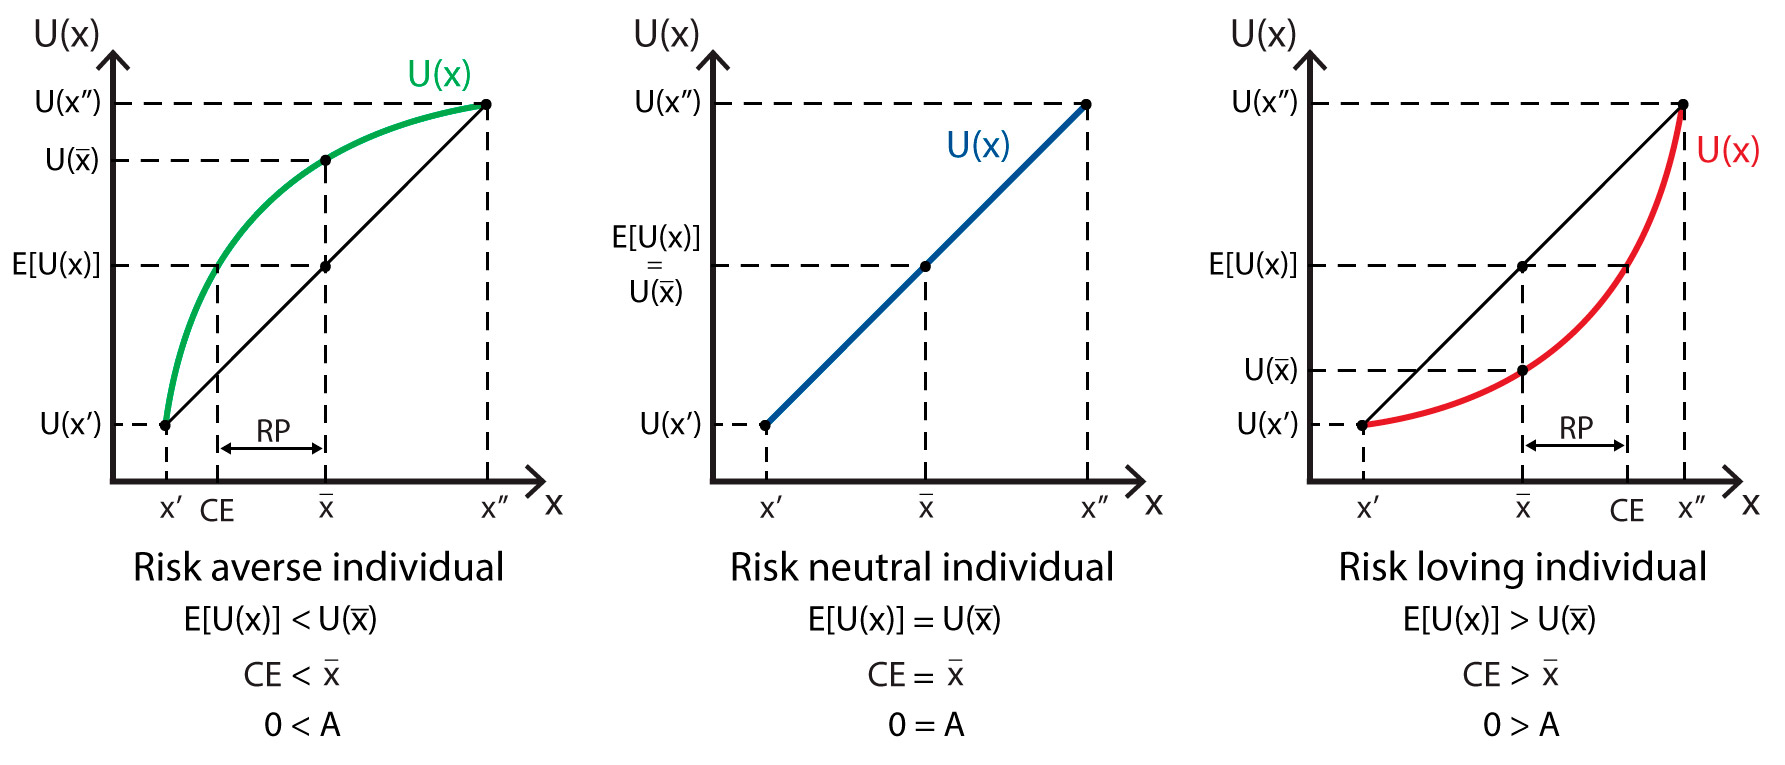
\includegraphics[scale = 0.25 ]{Risk-aversion.jpg}\\
$g = (\frac{1}{2} \circ w_1, \frac{1}{2} \circ w_2)$\\
$u(g) = \frac{1}{2} u(w_1) + \frac{1}{2} U(w_2)$\\
Below average than gable offered individual can be indifferent\\
$\Rightarrow$ Certainty Equivalent\\

$\bullet$ \textbf{Certainty Equivalent}\\
\[u(g) = U(CE) \,sure\, bet\]

$\bullet$ \textbf{Risk premium} 
\[ = E(g) - CE\]
Risk premium $>0$ if risk-averse\\
Risk premium $=0$ if risk-neutral\\
Risk premium $<0$ if risk-loving\\

\textbf{Arrow-Pratt measure of (Absolute) Risk-aversion}\\
Why not use degree of concavity as the measure of aversion? \\
$ u(\bar w) = \sqrt{w}, \, u''<0$ Immune to linear transformation\\
$ v(w) = 10\sqrt{w}, \, v'' = 10 u''$\\

\[R_a(w) = -\frac{u''(w)}{u'(w)} = constant \, r?\]
-- Immune to affine (linear) transformation of u(w)\\
-- $u(w) = -e^{(-rw)}$ (Constant absolute Risk aversion (CARA) Utility\\
$r_q(w)  = r\in [0, \infty)$\\
$\bullet$ \underline{Result}: Let $u(w) $ and $v(w)$ be twice differentiable VN-M utilities, with $u',v'>0$\\
Then if $-\frac{u''(w)}{u'(w)} > -\frac{v''(w)}{v'(w)}$ for all $w$, 
if and only if there is some function $h$ such that $ u(w) = h[v(w)],\,h'>0$ and $h''<0$\\
$\bullet$ \underline{Example}\\
$u(w) = w \rightarrow$ Risk-neutral ($\alpha w +\beta , \alpha >0$)\\
$v(w) =\sqrt{w}$\\
$\hat{v}(w) = ln (\sqrt{w})$\\
$\hat{\hat{v}}(w) = \sqrt{ln\sqrt{w}}$\\
\underline{Proof}:\\
($\Rightarrow$)$ h = v \circ v^{-1}$ (Notation: $f \circ g(x) = f [g(X)]$\\
Show that $h'>0, h''<0$\\
($\Leftarrow$) Suppose $u(w) = h[v(w)],h'>0, h''<0$\\
\\
$\bullet$\underline{Result}: Let u(w) and v(w) be twice differentiable VN-M utilities,\\
if $-\frac{u''(w)}{u'(w)} > -\frac{v''(w)}{v'(w)}$ for all $w$,then $CE_u< CE_v$\\
(Equivalent to Risk Premium for $u>$ Risk Premium for $v$)\\
\underline{Proof}:\\
By the previous result, $u(w) = h[v(w)]$, for some h such that $h'>0,h''<0$\\
Consider a gamble $g = (p_1\circ w_1, \cdots, p_n \circ w_n)$\\
$u(g) = \sum p_i u(w_i) = u(CE_u)$\\
Moreover, 
\begin{align*}
    \sum p_i u(w_i) &= \sum p_i h(v(w_i))\\
                    &< h(\sum p_i v(w_i))\\
                    &= h(v(CE_v))\\
                    &= u(CE_v)\\
\end{align*}
Aside: u(concave), $\sum p_i h(x_i) < h(\sum p_ix_i)$\\
Together, 
\[u(g) = U(CE_u) \le U(CE_v)\]
since u is strictly increasing ($u'>0$), we have $CE_u< CE_v$.\\
$\bullet$\underline{Example}: The demand for Insurance
$u_0$: initial wealth\\
p: prob of a loss, $L>0$\\
q: Insurance coverage in case of an accident\\
$\pi q$: premium paid to insurance   $\pi \in (0,1)$, fixed by the insurance company \\
Q: How much coverage q would a risk-averse person buy?
\begin{gather*}
    g = (p \circ (w_0 -L-\pi q+q), (1-p)\circ (w_0 - \pi q))\\
    max\limits_q \qquad p \, U(w_0 -L-\pi q+q) + (1-p)\, U(w_0 - \pi q) = u(g)\\
    FOC: \frac{\partial}{\partial q} = p(1-\pi) U'(w_0 -L-\pi q+q) -(1-p)\pi U'(w_0 - \pi q) = 0\\
    SOC: \frac{\partial^2}{\partial q^2} = p(1-\pi)^2 u''(w_0 -L-\pi q+q) -(1-p)\pi^2u''(w_0 - \pi q)\\
    p(1-\pi) U'(w_0 -L-\pi q+q) = (1-p)\pi U'(w_0 - \pi q)
\end{gather*}
Suppose it is a fair insurance: $\pi = p$ ( not fair $\pi > p \Rightarrow$ Under Insurance)
\[p(1-p) U'(w_0 -L-p q+q) = (1-p)p U'(w_0 - p q)\]
Since $u''<0, u'$ is strictly monotonic,\\
$ w_0 -L-\pi q+q = w_0 - \pi q \Rightarrow q* = L$    Full insurance.\\

$\bullet$\underline{Result}:Let u(w) be twice differentiable VN-M utility, consider a symmetric gamble $g= (\frac{1}{2}\circ (w+h), \frac{1}{2}\circ (w-h))$. Then, the risk premium $\pi(h) \approx r_a(w)h^2/2 $  for small $h>0$\\
\underline{Proof}:
Note that $E(g) = w$\\
By definition, $\pi(h) = E(g) - CE$\\
$\Rightarrow CE = w - \pi(h)$\\
Then, 
\begin{gather*}
    U(CE) = \frac{1}{2}U(w+h) +\frac{1}{2} U(w-h)\\
    U(w - \pi(h)) = \frac{1}{2}U(w+h) + \frac{1}{2}U(w-h)
\end{gather*}
$\pi(0) = 0$,next, differentiate both sides w.r.t h:
\[U'(w-\pi(h)) \pi'(h) = \frac{1}{2}U'(w+h) -\frac{1}{2} U'(w-h)\]
set $h = 0$, 
\[U'(w-\pi(0)) \pi'(0) = 0\quad\Rightarrow \pi'(0) = 0\]

Differentiate w.r.t. h once more, 
\[U''(w-\pi(h)) [\pi'(h)]^2 +U'(w-\pi(h)) (-\pi''(h))  = \frac{1}{2}U''(w+h) + \frac{1}{2} U''(w-h)\]
Set $h = 0$, and recall $\pi(0) = \pi'(0) = 0$
\begin{gather*}
    u'(w)(-\pi''(0)) = u''(w)\\
    \pi''(0) = -\frac{u''(w)}{u'(w)}
\end{gather*}
By Taylor's expansion,
\[\pi(h) = \pi(0) +\frac{\pi'(0)}{1!}h + \frac{\pi''(0)}{2!}h^2 + \dots + \frac{\pi^{(n)}(0)}{n!}h^n\]
(The rest is less important than first two term and since the first two term equal 0, the third is most important)
\[\pi(h) = \frac{\pi''(0)}{2}h^2 = r_a(w) \frac{h^2}{2}\]
\textbf{Arrow-Pratt Measure of Relative Risk-aversion}
\[r_r(w) = -\frac{u''(w)}{u'(w)}w\]
$\bullet$\underline{Result}: Consider a "percentage" gamble, 
\[g = (\frac{1}{2} \circ (w+hw), \frac{1}{2}\circ(w-hw))\]
Then the percentage risk premium at g is 
\[ \pi(h) = r_r(w)\frac{h^2}{2}\]
Constant Relative risk Aversion(CRRA)\\
\[
    u(w)=\left\{
            \begin{array}{ll}
                 &\frac{ w^{1-\varrho} -1}{1-\varrho} , \varrho \in (0,1)\\
                 & ln w, \varrho = 1
            \end{array}
            \right
\]

\[r_r(w) = \varrho\]

why not $\hat{u}(w) = w^{1-\varrho}$?\\
Problem on limit when $\varrho =1, \hat{u}(w) = 1$ but actually it should approach $lnw$, but for the one in equation, when $\varrho=1, \frac{0}{0}$, unreachable\\
\\
\textbf{Relation between CARA and CRRA}\\
If CARA(i.e. $r_r(w) = \varrho$), Then 
\[r_a(w) = \frac{\varrho}{w}\]
In particular, CRRA $\Rightarrow$ Decreasing Absolute Risk Aversion(DARA) because $r_a(w) = \frac{\varrho}{w} \downarrow $ in w\\
(Percentage is constant, but $w \uparrow$, then in absolute term , win& loss becomes larger)\\
CARA: $u(w) = -e^{-rw}, r>0$\\
(Increase w, the one gives up same dollar to avoid risk)\\
$g = (\frac{1}{2} \circ (w+h), \frac{1}{2}\circ (w-h)$\\
(e.g. w from \$100 to 100 million, h unchanged at \$5 for CARA)\\
CARA $\Rightarrow$ increasing relative risk aversion ($r_r(w) = -\frac{u''(w)}{u'(w)}w \uparrow$)\\

\underline{Implication}\\
gamble $\Rightarrow \tilde{w}$\\
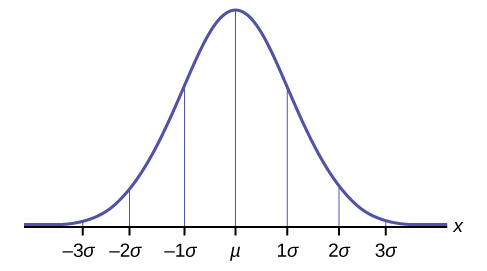
\includegraphics{normal.jpg}\\
$E u (\tilde{w}) =$ (mean, variance)\\
$\bullet$ Mean-variance Expected Utilities\\
\underline{Idea1}: 
\begin{gather*}
    u(w) = w-bw^2, b>0\\
    E u(\tilde{w}) = E \tilde{w} - b E(\tilde{w}^2) = \mu - b(\sigma^2 +\mu^2) \\
    ( E(\tilde{w}^2) = \sigma^2 +\mu^2)
\end{gather*}
Nice but $u'>0 $ (not everywhere)\\
\underline{Idea2}:CARA-Normal Model
\begin{gather*}
    u(w) = -e^{-rw},\tilde{w}\sim Normal(\mu, \sigma^2)\\
    E U(\tilde{w}) = -\int e^{-rw}f(w)dw\\
                  = -e^{-r(\mu - \frac{r}{2}\sigma^2)} = -e^{-rCE}\\
    E U(\tilde{w}) = U(CE)
\end{gather*}
\textbf{Paradox}\\
Axioms$\Rightarrow$ U(q) + Independence Axiom
 $\Rightarrow$ Expected Utility\quad 
            $U(g) = \sum\limits_{i}p_iu(w_i)$\\
\begin{center}
A: \$ 1 million for sure \\
B: 5 million with prob 90\%\\
    nothing with prob 10\%\\
C: \$ 1 million with prob 10\%\\
    nothing with 90\%\\
D: \$ 5 million with 9\%\\
    nothing with 91\%\\
\end{center}
Note that $C = 10\% A +90\% (0), D = 10\%B + 90\%(0)$\\
If $A\succeq B$, then Independence $\Rightarrow C\succ D$\\
(However, the difference with reality is not about risk. It is behavior paradox.) \\

Let u be VN-M utility for the individual, \\
\underline{The Allias Paradox}\\
$A\succ B\Leftrightarrow u(1) \succ 0.9 u(5) +0.1 u(0)$\\
$D \succ C \Leftrightarrow 0.09 u(5) + 0.91 u(0) > 0.1 u(1) +0.9 u(0)$\\
\underline{Rabin's Paradox}\\
$g = (0.6\circ \$5, 0,4 \circ (-\$5))$ Really risk-averse to avoid loss of \$5\\
$g'= ((0.6\circ \$1 \,billion, 0,4 \circ (-\$200))$ The same person should not take  with more loss\\
(Prospect theory: more sensitive to loss than gains)\\
(Preference in small gamble is not utilized to big gamble)\\
\includegraphics[scale = 0.08]{graph/rabinparadox.png}
\newpage
\section{Production and Cost}
\subsection{Production}
\[nput\begin{array}{*{20}{c}}
{{x_1}}\\
 \vdots \\
{{x_n}}
\end{array}\begin{array}{*{20}{c}}
 \to \\
{}\\
 \to 
\end{array}\begin{array}{*{20}{c}}
{firm}\\
\fbox{f}\\
{"Black \,box"}\\

\end{array} \to q(output)\]
\begin{center}
    {Production}\\
    {$q = f(x_1,\dots,x_n)$}\\
    {     $\uparrow$ Production function}\\
\end{center}
$\bullet$ Assumptions: \[f: R^n_+ \rightarrow R_+\]
is continuous strictly increasing and $f(0) = 0$\\
$\bullet$ \textbf{Productivity measure of inputs}\\
\begin{enumerate}
    \item Average product of input i:
    \[AP_i = \frac{q}{x_i}\]
    \item Mariginal product of input i:
    \[MP = \frac{\partial f}{\partial x_i}\]
    \item Returns to scale (Joint Productivity of Inputs)\\
    f(x) has:
    \begin{enumerate}
        \item  Constant returns to scale (CRS)\\
         if $f(tx) = t(f(x)), \forall t>0$\\
         (Equivalent to f(x) is HD1 in x)
         \item Increasing returns to scale (IRS)\\
         $f(tx) >tf(x), t>1$
         \item Decreasing returns to scale (DRS)\\
         $f(tx)<tf(x), t>1$\\
    \end{enumerate}

\end{enumerate}
\underline{Example}
\[f(x_1,\dots,x_n) = x_1^{\alpha_1}\,x_2^{\alpha_2}\dots x_n^{\alpha_n}, \alpha_i>0\]
f has CRS if $\sum \alpha_i = 1$\\
f has IRS if $\sum \alpha_i > 1$\\
f has DRS if $\sum \alpha_i < 1$\\
\underline{NOTE}: The topic and cost is similar to consumer theory except:
\begin{enumerate}
     \item Unlike utility function, f is cardinal (i.e. quantity matters)
     \item No budget constraint (Only substitution)\\
         (i.e. No income effect)
\end{enumerate}
\\
$\bullet$\textbf{Iso-quants}\\
\includegraphics[scale = 0.1]{graph/isoquant.png}
\[    f(x_i,x_j,x_{-ij}) = q \,\, (x_{j} = (x_i,x_{-ij}))\]
\[\frac{\partial f}{\partial x_i} +\frac{\partial f}{\partial x_j}\frac{\partial x_j}{\partial x_i} = 0\]
\[\Rightarrow {\left. {\frac{\partial x_j}{\partial x_i}} \right|_q} = -\frac{\partial f/\partial x_i}{\partial f/\partial x_j}\]
\begin{align*}
        MRTS_{j,i} &= -\left. {\frac{\partial x_j}{\partial x_i}} \right|_q\\
        &=\frac{\partial f/\partial x_i}{\partial f/\partial x_j} = \frac{MP_i}{MP_j}
\end{align*}

\underline{Result}: If f(x) is quasi-concave, them $MRTS_{j,i}$ is diminishing\\
$\bullet$\textbf{Quasi-concavity}
\begin{enumerate}
    \item $f(\alpha x+(1-\alpha)x') \ge min\{f(x),f(x')\}$
    \item $\{x|f(x) \ge q\}$ is convex.
    \item Bordered Hessian Matrix\\
    \newline
$B =$ 
\begin{bmatrix}
 &0 &f_1  &\dots &f_n \\ 
 &f_1  &f_{11}  &\dots &f_{1n} \\ 
 &\vdots  &\vdots  &\vdots &\vdots \\ 
 &f_n  &f_{n1}  & \dots &f_{nn} 
\end{bmatrix}
\qqad $\frac{\partial f}{\partial x_i} = f_i$ \qquad
$\frac{\partial ^2 f}{\partial x_i \partial x_j} = f_{i,j}$\\
quasiconcave if 
\begin{vmatrix}
 &0 &f_1 \,\\
 &f_1 &f_{11}\,\\
\end{vmatrix}\le 0, 
\begin{vmatrix}
 &0 &f_1 &f_{11}\,\\
 &f_1 &f_{11}&f_{12} \,\\
 &f_2 &f_{21} &f_{22}\,\\
\end{vmatrix} \ge 0,
\begin{vmatrix}
 &0 &f_1 &f_{11}\,\\
 &f_1 &f_{11}&f_{12} \,\\
 &f_2 &f_{21} &f_{22}\,\\
  &f_3 &f_{31} &f_{33}\,\\
\end{vmatrix} \le 0

\end{enumerate}
\\
$MRTS_{j,i}$ is not unit free. \\
$\bullet$\textbf{The Elasticity of Substitution}
\[= \sigma_{j,i}\]
\[= \frac{d(x_j/x_i)/(x_j/x_i)}{d(MRTS)_{j,i}/(MRTS)_{j,i}}\]
\[\cong \frac{\text{$\%$ change in $x_j/x_i$}}{\text{$\%$ change in $(MRTS)_{j,i}$}}\]
\[= \frac{dln(x_j/x_i)}{dln((MRTS)_{j,i})}\]
\underline{Example}:
\begin{gather*}
    f(x) = [\sum\limits_{k=1}^{n}(\alpha_kx^\varrho)]^{\frac{1}{\varrho}}, \sum \alpha_k >0, \varrho <1 (quasi-concave)\\
    \frac{\partial f}{\partial x_i} = f_i = 1/\varrho(\sum(.))^{\frac{1}{\varrho}-1} \alpha_i\varrho \,x_i^{\varrho-1}\\
    \frac{\partial f}{\partial x_j} = f_j =  1/\varrho(\sum(.))^{\frac{1}{\varrho}-1} \alpha_j\varrho \,x_j^{\varrho-1}\\
\end{gather*}
\begin{gather*}
    MRTS_{j,i} =-\left. {\frac{\partial x_j}{\partial x_i}} \right|_q= \frac{f_i}{f_j}\\
    MRTS_{j,i} = \frac{\alpha_i}{\alpha_j}(\frac{x_j}{x_i})^{1-\varrho}\\
    ln(MRTS_{j,i}) = ln (\alpha_i/\alpha_j) +(1-\varrho)ln(x_j/x_i)\\
    \sigma_{j,i} = \frac{dln(x_j/x_i)}{dln(MRTS_{j,i})} = \frac{1}{1-\varrho}\quad \text{Independent of $x_i,x_j$ (Constant $\rightarrow$ CES)}
\end{gather*}  
\begin{center}
    As $\varrho \uparrow, \sigma_{j,i} \,\uparrow$ 
\end{center}
Special Case:\\
\varrho \rightarrow1, f=\sum \alpha_kx_k\\
\varrho\rightarrow -\infty, f=min\{x_1,\dots,x_n\}\\
$\varrho\rightarrow0, f=\prod\limits_{i}x_i^{\alpha_i}$, Cobb-Douglas,substitution but not perfect substitute\\
CES $\rightarrow$ CRS
\begin{align*}
f(tx) &= (\sum \alpha_k(tx_k)^\varrho)^{\frac{1}{\varrho}}\\
&=tf(x)
\end{align*}
\[g(x) = f(x)^2 \Rightarrow IRS (t>1)\text{   ( Monotonic transformation doesn't work now )}\]

\subsection{Cost}
Assume that firm take input prices as given(Small firm have no power in market and no effects on wages)
\begin{gather*}
    w=(w_1,\dots,w_n)\\
    C(w,q) = min\limits_{x_1,\dots\,x_n} \quad w\bullet x = \sum w_ix_i\\
    s .to \quad f(x) \ge q \,\text{(fixing output)}\\
    \Rightarrow \bar{x}(w,q) -\text{ conditional input demand(Unique solution)}\\
    C(w,q) = w\bullet \bar{x}(w,q) \\
    \uparrow \text{(Cost Function)}
\end{gather*}
\newpage
$\bullet$ \textbf{Properties of C(w,q)}
\begin{enumerate}
    \item Continuous in (w,q) [f is continuous](From $f(x) \ge q$ Don't need to be quasi-concave)
    \item Increasing in w and q [Follow from the Envelope Thm]
    \item HD1 in w
    \item concave in w
    \item$\bar{x}(w,q) = \frac{\partial C}{\partial w_i}$  [Follow from the Envelope Thm]
\end{enumerate}
$\bullet$ \textbf{Properties of $\bar{x}$(w,q)}\\
Assume f is strictly quasi-concave ( $\bar{x}(w,q)$ is unique )
\vspace{50mm}\\
$w_1x_1+w_2x_2 = C$ -- iso-cost line
\begin{enumerate}
    \item Continuous in (w,q)\\
    (Small changes correspond to small result, x change smoothly or it is not continuous.Input jumps easily but cost not.)\\
    e.g.\\
    $\bullet$ Berge's theorem of the maximum\\
    $f(x) = max \{x_1,x_2\}$ Not quasi-concave
    \begin{gather*}
        \limits{min}_{x_1,x_2}\quad w_1x_1 +w_2 x_2\\
         s.to f(x_1,x_2)\ge q\\
          \bar{x}_i=\left\{
            \begin{array}{ll}
                 &q \qquad\,if\,w_i<w_j\\
                 &\{0,q\}\quad\,if\,w_i=w_j\\
                 &0\qquad\, if\,w_i>w_j
            \end{array}
            \right
    \end{gather*}
    $\bar{x_i}$ jumps, but cost doesn't.
  
    \begin{equation*}
    \begin{rcases}
         w_1 = 1\\
        w_2 = 1-\epsilon
    \end{rcases}
    \bar{x}_2 = q \qquad 
    \bar{x}_1 = 0
    \Rightarrow C=(1-\epsilon)q
    \end{equation*}

    \begin{equation*}
    \begin{rcases}
         w_1 = 1\\
        w_2 = 1+\epsilon
    \end{rcases}
    \bar{x}_2 = 0 \qquad 
    \bar{x}_1 = q
    \Rightarrow C= q
    \end{equation*}
    
\end{enumerate}


\subsubsection{Relationship between Production Function \& Cost}
Suppose f(x) is HDk, $k>0$, in this case
\[C(w,q) = C(w,1)q^{1/k}\]
Proof:
\begin{gather*}
    min\limits{x}  \quad w\bullet x \\
    s.to\quad \frac{f(x)}{q} \ge \frac{q}{q}\\
    \Updownarrow\\
    min\limits{x}  \quad w\bullet x \\
    s.to \quad \frac{1}{q}f(x)\ge1\\
    f(\frac{1}{q^{1/k}}x)\ge1\\
    x\\
    (f(tx) = t^kf(x) = \frac{1}{q}f(x))
\end{gather*}
\begin{enumerate}
    \item For $k=1$, f has CRS. \\
    $\Rightarrow C(w,q) = C(w,1)q \Rightarrow \frac{\partial c}{\partial q} = C(w,1) = $constant
    \item For $k>1$, \\
    $f(tx) = t^kf(x) >tf(x)$, for $t>1$\\
    $\Rightarrow$ IRS\\
    $\frac{\partial C}{\partial q} = \frac{1}{k}q^{\frac{1}{k}-1} C(w,1)$\\
    Let $k =2, \frac{\partial C}{\partial q} = \frac{1}{2}q^{\frac{1}{2}}C(w,1), \downarrow$ in q.
    \item For $k<1\Rightarrow$ DRS $\Rightarrow \frac{\partial C}{\partial  q } \uparrow $ in q.\\
\end{enumerate}
CRS $\Rightarrow$ Constant MC\\
IRS $\Rightarrow$ Decreasing MC\\
DRS $\Rightarrow$ Increasing MC\\
\\
\underline{Example}:\, $C(q) = q^2, MC = 2q, \uparrow$ in q $\Rightarrow$ DRS\\

$\bullet$ \underline{Average Cost}\\
\[AC = \frac{C(w,q)}{q}\]
\[\frac{\partial AC}{\partial q} = \frac{\partial C/\partial q - C}{q^2} = \frac{MC -AC}{q}\]

If $MC > AC$, AC $\uparrow$\\
If $MC < AC$, AC $\downarrow$\\
If $MC = AC$, AC constant.\\
\includegraphics[scale = 0.05]{graph/mcac.png}
\includegraphics[scale = 0.05]{graph/mcac2.png}
\subsubsection{Short v.s Long-run Cost}
$x = (x_0, x_1) \quad w= (w_0,w_1)$\\
$x_1$ fixed, $\leftarrow$ short-tun (some inputs are fixed)
\begin{gather*}
    min\limits_{x_0} \quad w_0x_0 +w_1x_1\\
    s.to\qquad f(x_0,x_1)\ge q\\
    \Downarrow\\
    \hat{x}_0 = \hat{x}_0 (w,q,x_1)\\
    SC(w,q,x_1) = w_0 \hat{x}_0(w,q,x_1) + w_1 x_1\\
    \text{   \qquad variable cost \qquad \quad  fixed cost (w.r.t. q)}
\end{gather*}
In the long run, 
\begin{gather*}
    C(w,q) = min\limits_{x_1}\, SC(w,q,x_1) \Leftrightarrow \, min\limits_{x_1}\,(min\limits_{x_0} \, w_0x_0 +w_1x_1)\\
    \qquad s.to f(x_0,x_1)\ge q\\
    \bar{x}_1 = \bar{x}_1(w,q)\quad 
    \bar{x}_0 = \hat{x}_0(w,q,\bar{x}_1) = \bar{x}_0(w,q)\,\Leftrightarrow \, min\limits_{x_1, x_0}\, w_0x_0 + w_1x_1\\
    s.to \, f(x_0,x_1) \ge q
\end{gather*}
\underline{Aside}: \[min\limits_{x,y}\, f(x,y) \Leftrightarrow min\limits_{y}\, min\limits_{x}\, f(x,y) \]
Order doesn't matter.\\
\\
$C(w,q) \le SC(w,q,x_1)$\\
$\hat{x}_0(w,q,x_q) > < \bar{x}_0(w,q)$\\
Long-run cost is no greater than short-run cost. There is no exact relationship between short-run and long-run variable input.
Conclusion: In the short run, depending on fixed inputs, variable inputs may be chosen suboptimally -- i.e. they may not be cost minimizing in the long run\\
$MRTS_{j,i} \ne w_j/w_i$\\
\underline{Example}:
\[f(x) = x_1^{\frac{1}{2}}x_2^{\frac{1}{2}}\]
Long run: 
\begin{gather*}
    min\limits_{x_1, x_2} \, w_1x_1 +w_2x_2\\
    s.to \quad x_1^{\frac{1}{2}}x_2^{\frac{1}{2}} \ge q \,\, (=, \text{since }w_1,w_2 > 0 )\\
    \Downarrow\\
    \bar{x}_1 = \sqrt{\frac{w_2}{w_1}}\,q, \, \bar{x}_2 = \sqrt{\frac{w_1}{w_2}}\,q\,\,, C(w_1,w_2,q) = 2\sqrt{w_1w_2}\,q
\end{gather*}
Short run, $x_2$ fixed
\begin{gather*}
    min\limits_{x_1} \, w_1x_1 +w_2x_2\\
    s.to \quad x_1^{\frac{1}{2}}x_2^{\frac{1}{2}} \ge q \quad \Rightarrow \hat{x}_1 = \frac{q^2}{x_2}\\
    SC = w_1 \frac{q^2}{x_2} + w_2x_2\\
    \frac{\partial SC}{\partial q} = 2w_1 \frac{q}{x_2}, \,\, \uparrow \text{ in q}\\
    \text{(May conclude DRS, which is not right!)}
\end{gather*}
  (Return to scale = double all inputs. But in short tun, some input is fixed.\\So short run is not good way to understand technology.)\\
Find long-run cost(knowing SC)
\begin{gather*}
    min \limits_{x_2}\, SC\\
    FOC:\quad \frac{\partial SC}{\partial x_2} = -w_1 \frac{q_2^2}{x_2^2} + w_2 = 0\\
    \Rightarrow x_2 = \sqrt{\frac{w_1}{w_2}\,q}\\
    C(w,q) = 2\sqrt{w_1 w_2}\,q\\
    \frac{\partial C}{\partial q} = 2\sqrt{w_1 w_2} = \text{constant $\Rightarrow$ CRS}
\end{gather*}
 \subsubsection{Cost with multiple plants}
 \begin{center}
 \fbox{HQ} $\leftarrow Q$ units\\
 \downarrow q_1 \qquad \downarrow q_2\\
 \fbox{Plant1}\qquad \fbox{Plant2}\\
 $f_1,w_1\qquad f_2,w_2$
 \end{center}
 \underline{Example1}:\\
 $c_1(q_1) = 2q_1^2 \leftarrow $ DRS\\
 $c_2(q_2) = q_2^2 \leftarrow $ DRS\\
 What is the cost function of whole company, C(Q)?
 \begin{gather*}
 min\limits_{q_1,q_2}\,C_1(q_1) + C_2(q_2)\\
 s.to \quad q_1 + q_2 = Q\\
 \Leftrightarrow \, \,min\limits_{q_1, q_2} \, 2q_1^2 + q_2^2 \quad \Leftrightarrow \,\, min\limits_{q_1}\, 2q_1^2 + (Q-q_1)^2\\
 s.to \quad q_1+q_2 = Q\\
 FOC: \frac{\partial }{\partial q_1} (.) = 4q_1 - 2(Q- q_1) = 0\\ \Rightarrow \, q_1 = \frac{Q}{3}\quad q_2 = \frac{2Q}{3}\\
 SOC: \frac{\partial^2 }{\partial q^2}(.) = 6>0\, (OK)\\
 C(Q) = \frac{2}{3}Q^3
 \end{gather*}
 \underline{Example 2}:
 \begin{gather*}
     c_1(q_1) = q_1 \,(CRS) \quad c_2(q_2) = q_2^2 \,(DRS)\\
     min \limits_{q_1,q_2} \,\, q_1 + q_2^2 \Leftrightarrow \quad min\limits_{q_1} \, q_1 + (Q- q_1)^2\\
     s.to\quad q_1+q_2 = Q\\
     FOC: \frac{\partial}{\partial q_1} (.) = 0 \,\Rightarrow \, q_1 = Q-\frac{1}{2} \Rightarrow q_2 = \frac{1}{2}\\
     SOC: \frac{\partial ^2}{\partial q_1^2}(.) = 2>0 (OK)\\
     \text{If } Q<\frac{1}{2,}, \, q_1= Q-\frac{1}{2}< 0 (no)\\
     \Rightarrow q_1 = 0\, \Rightarrow q_2 = Q \\
     \text{If } Q \ge \frac{1}{2}, q_1 = Q - \frac{1}{2} \ge 0, q_2 = \frac{1}{2}\\
     C(Q) =\left\{
            \begin{array}{ll}
                 &Q^2 \qquad if\, Q<\frac{1}{2}\\
                 &Q - \frac{1}{4}\quad if\, Q\ge\frac{1}{2}
            \end{array}
            \right
    \\
     \text{Small Q choose DRS, large Q choose CRS(because at first $q_1 > q_2^2)$}  
  \end{gather*}
 \newpage
 \subsection{Profit Maximization and Supply Function}
 
 $\bullet$ Assumtpion: The firm takes price as given.
 \begin{align*}
 max\limits_{x,q} \quad \pi &= pq - w\bullet x\\
 s\, to\quad f(x) &\ge q \rightarrow\, \text{binding since f(x) is strictly incresing}\\
 max\limits_{x}\quad \pi &= pf(x) - w\bullet x\\
 &\Downarrow\\
 x^*&= x^*(p,w) \rightarrow \text{Unconditional input demand}\\
 \Downarrow\\
 q^*&=f(x^*)
 \end{align*}
 
 $\bullet$ \underline{Result}: $x^*(p,w)$ minimizes $w \bullet x$ s.to $f(x)\ge q^*$ \qquad [Profit max $\Rightarrow$ Cost min]\\
 \underline{Proof}: Suppose not. Then, there is some $x'\ne x^*$ that gives a lower cost to produce $q^*$
     \[w\bullet x'<w\bullet x^*\]
     Since $x^*$ is profit-max
     \begin{align*}
         pf(x^*) - w\bullet x^* &\ge pf(x') - w\bullet x'\\
         &\ge pf(x^*) - w\bullet x' [\text{Since $f(x') \ge f(x^*)$}]\\
         &>pf(x^*) - w\bullet x^*
     \end{align*}
     A contradiction. Hence $x' = x^*$.\\
$\bullet$ A two-step approach to profit max
\begin{enumerate}
    \item (fix q, minimize cost)\\
    Given q, 
    \begin{gather*}
        min\limits_{s}\quad w\bullet x\\
        s.to \quad f(x) \ge q\\
        \Downarrow\\
        C(w,q)
    \end{gather*}
    \item (fixed cost, maximize profit)\\
    Given C(w,q)
   \begin{align*}
       & max\limits_{q}\quad \pi = pq- C(w,q)\\
       FOC: \, \frac{\partial \pi}{\partial q} &= p-\frac{\partial c}{\partial q} = 0 \Rightarrow MC(q,w) \Rightarrow q^*(p,w) \text{  (Supply Function)}\\
       SOC: \, \frac{\partialL^2 \pi}{\partial q^2} &= -\frac{\partial^2 c}{\partial q^2}<0 \Rightarrow \frac{\partial MC}{\partial q}>0 \text{ (Only exist when DRS)}
   \end{align*}
   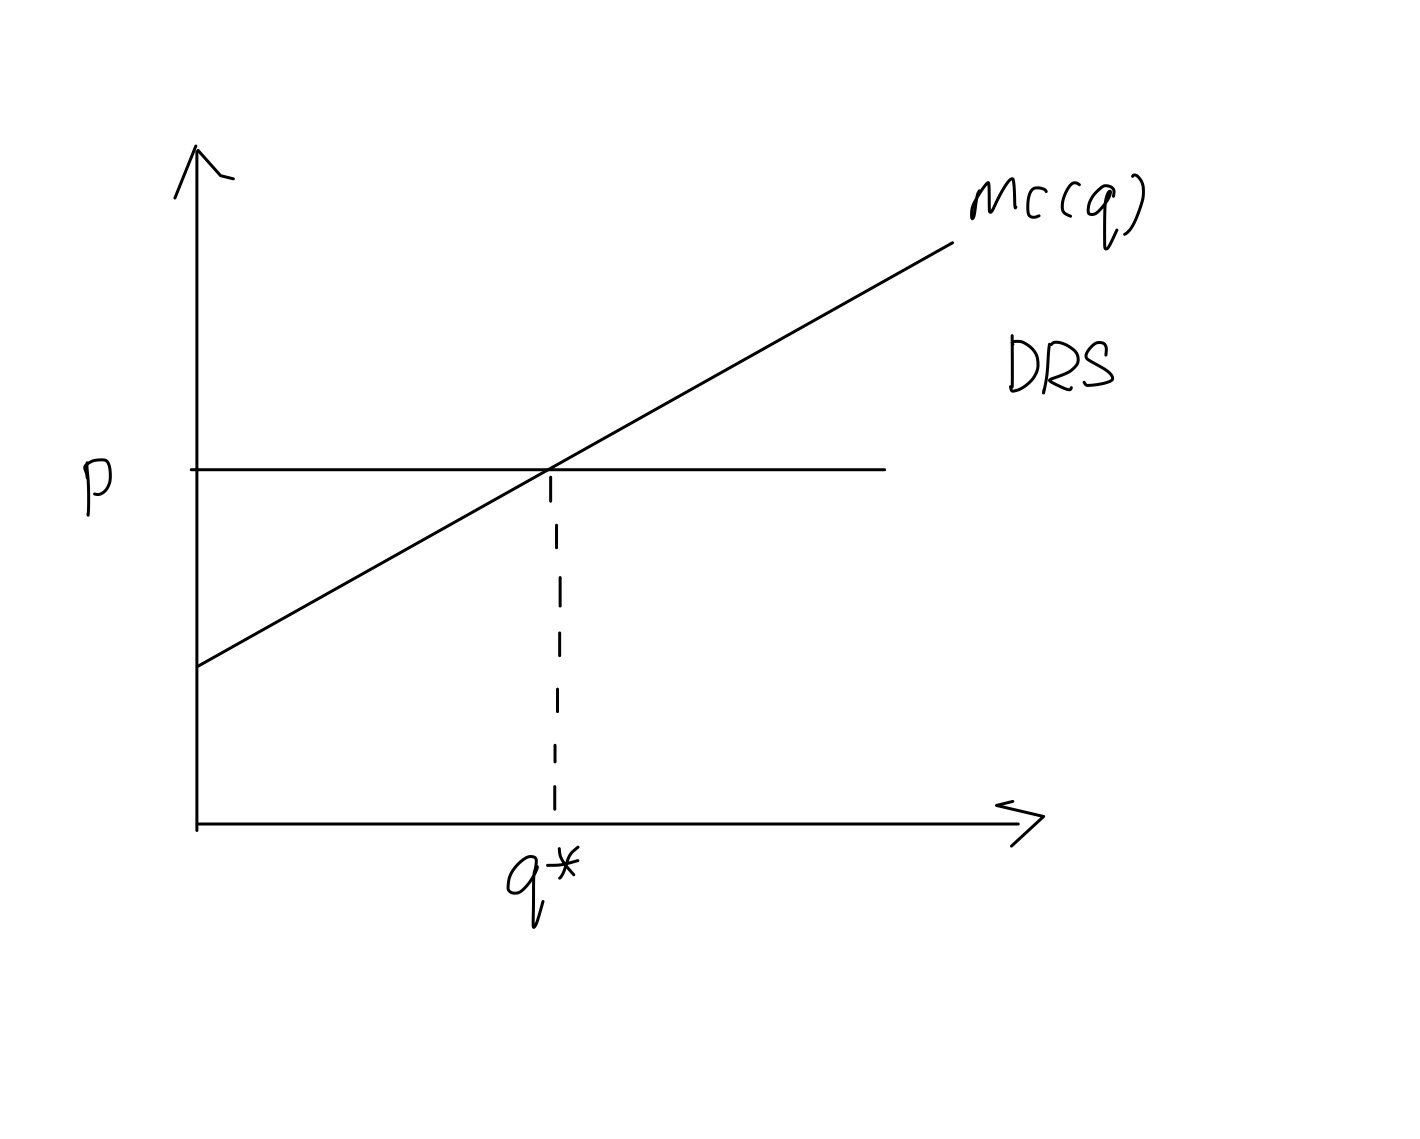
\includegraphics[scale = 0.2]{approach-to-max-profit.jpg}
\end{enumerate}
What if the firm has CRS or IRS?\\
CRS $\Rightarrow \, C(w,q) = C(w,1)q \rightarrow x= pq-c = (p-c(w,1))q \Rightarrow q^* = 0, \infty $\\
( $p>MC, \infty ; p = MC, q \text{ is undetermined}\,(0 \, ,\infty) ; p< MC, 0$)\\
IRS $\Rightarrow \, q^* = \infty$
\begin{gather*}
    \Pi(p,w) = max\limits_{q} \, \pi = pq - C(w,q)\\
    \Downarrow\\
    q^*(p,w)
\end{gather*}
By Shephard's Lemma, $\bar{x}_i(w,q) = \frac{\partial c}{\partial w} \Rightarrow x_i^* = \bar{x}_i(w,q^*)$\\

$\bullet$Property of $\Pi(p,w)$\\
\begin{enumerate}
    \item $\Pi(p,w)$ is increasing in p, and decreasing in $w_i$.\\
    Proof: By the Envelope Theorem. 
    \[\left. \frac{\partial \pi}{\partial p}\right |_{q^*}= q|_{q^*} = q^* \ge 0\]
    \[\left.\frac{\partial \pi}{\partial w_i}\right |_{q^*} = -\left.\frac{\partial C}{\partial w_i}\right |_{q^*} = -\left. \bar{x}(w,q)\right |_{q^*} = -x^*(w,p) \le 0\]
    \item $\Pi(p,w)$ is HD1 in (p,w)\\
    ($\pi(p,w) = max\limits_{q}\quad \pi = tpq - C(tw,q)$)
    \item $\Pi(p,w)$ is convex in (p,w)\\
    ($\Pi(p,w) = max_{\limits{q}} \, \pi = pq- C(w,q)$(concave in w))
    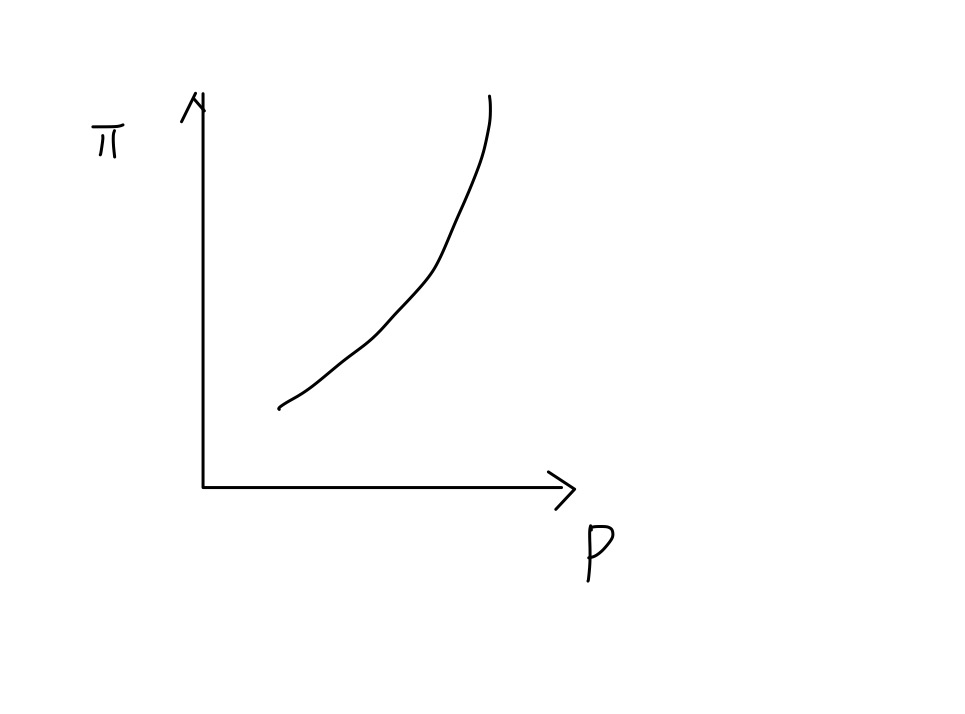
\includegraphics[scale = 0.15]{property-profit.jpg}\\
    Proof: Take\begin{gather*}
        (p',w')\rightarrow q'\\
        (p'',w'')\rightarrow q''\\
        (p^t,q^t)\rightarrow p_t = tp' +(1-t)p''; w_t = tw' +(1-t)w'' \rightarrow q^t
    \end{gather*}
    WTS: \[\Pi(p_t,w_t)\le t\,\Pi(p',w') +(1-t)\,\Pi(
    p'',w'')\]
    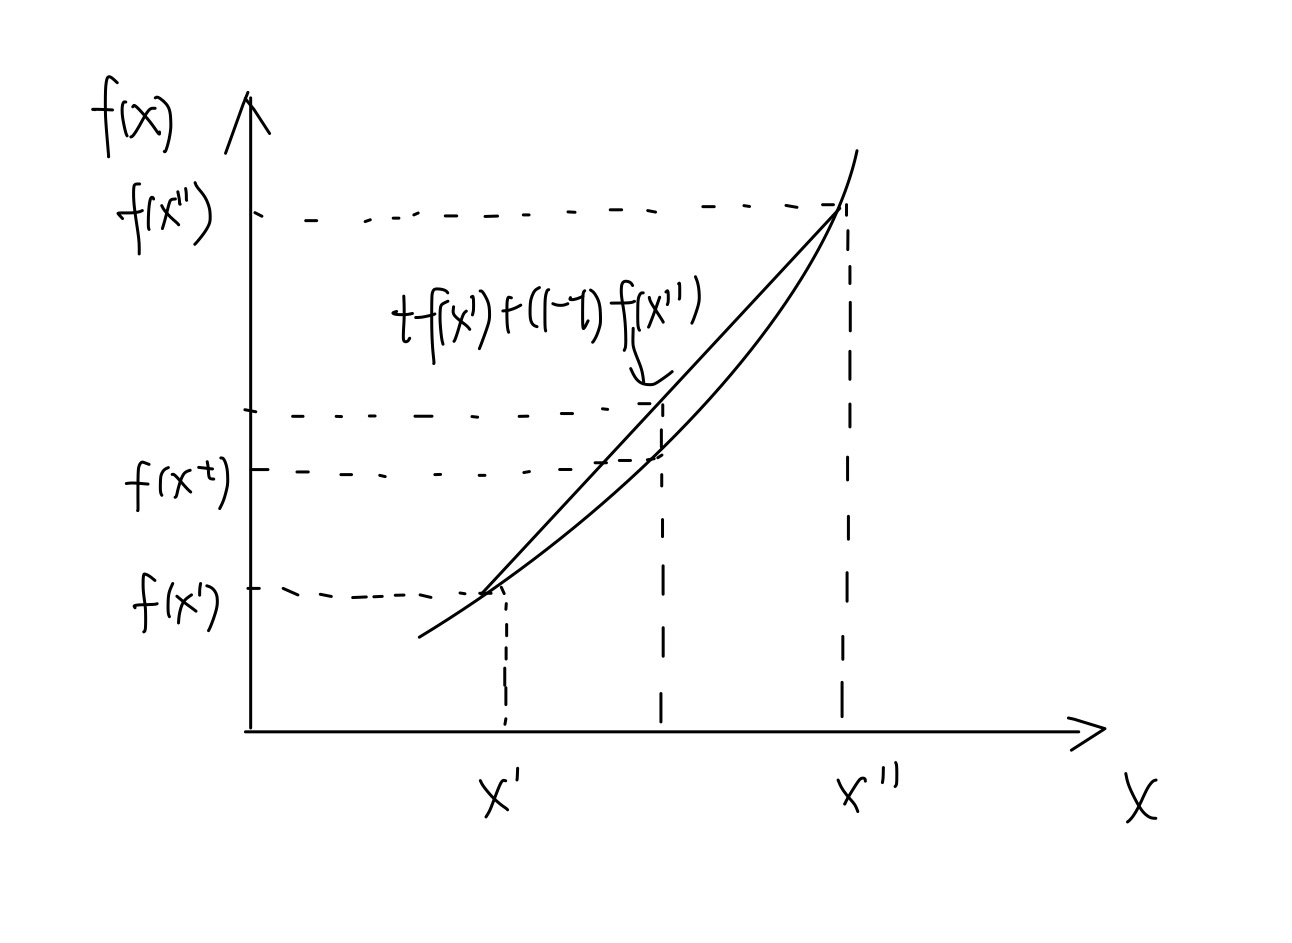
\includegraphics[scale = 0.2]{proof-convex.jpg}\\
    It means $\Pi(p,w)$ is convex in p.\\(It is convex in (p,w) so it is convex in p and w separately)\\
    convex $\Pi(p,w) \Rightarrow \partial^2 \Pi/\partial p^2 \ge 0, \partial^2 \Pi/\partial w_i^2 \ge 0$
    \begin{align*}
        \frac{\partial^2 \Pi}{\partial p^2} 
        &= \frac{\partial }{\partial p}(\frac{\partial \Pi}{\partial p})\text{ (Don't consider IRS &CRS when $q^*$ doesn't exist.)} \\
        &=\frac{\partial q^*}{\partial p}\ge 0\quad \text{(Non-decreasing supply curve)}
    \end{align*}
\end{enumerate}
\underline{Example}
\begin{align*}
    f(x_1.x_2) &= x_1^{\frac{1}{4}}x_2^{\frac{1}{4}}\\
    \Rightarrow C(w_1,w_2,q) &= 2\sqrt{w_1w_2}q^2\\
    max\limits_{q} \quad \pi &= pq-C(w_1,w_2,q)\\
    &\Downarrow\\
    q^*&= \frac{p}{4\sqrt{w_1w_2}}\quad \text{(Supply Function)}\\
    \Pi(p,w) &= \frac{p^2}{8\sqrt{w_1w_2}}
\end{align*}
\newpage
\section{General Equilibrium}
\subsection{A Pure Exchange Economy}
Partial Equilibrium: focus on one market while keeping all others fixed. \\$\rightarrow$ marshallian demand $x^*(P,I) \quad p_2,\dots,p_n $ fixed\\

$N = \{1,2,\dots,N\}$- the set of consumers\\
$\,\{1,2,\dots,k\}$-the set of goods\\

$w_i^j=$ consumer i's initial endowment of good j\\
$w_i = (w_i^1,w_i^2,\dots,w_i^n) \in R^k_+$ 

For all consumers, $\varepsilon = (\succeq_i, w_i)_{i\in N}$ [Assumer Consumer has utility function (Actually not necessary)] \qquad \qquad \quad \,$u^i$\\
$\bullet$ Feasible Allocations
\begin{align*}
    &F(w) = \{x \in R_+^{nk}|\sum\limits_{i\in N} x_i \le \sum\limits_{i\in N}w_i\} \\
    &\downarrow \qquad \qquad \qquad \qquad \downarrow\\
    &(w_1,\dots,w_n)\qquad \sum\limits_{i\in N} x_i^j \le \sum\limits_{i\in N}w_i^j,\forall j=1,\dots, k
\end{align*}

Special case: n=2, k=2\\
Edgeworth box\\
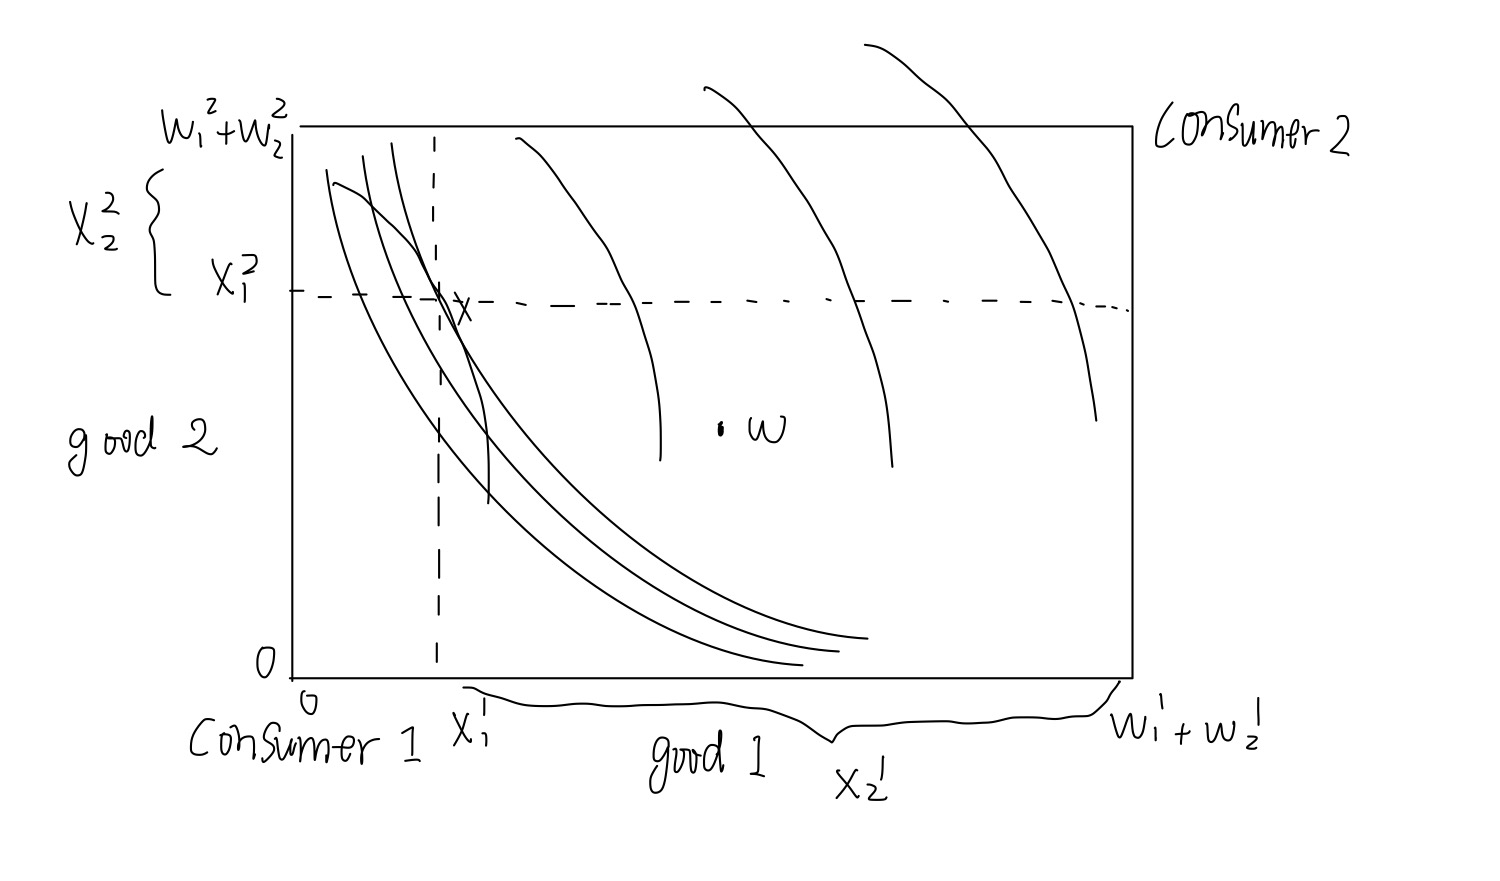
\includegraphics[scale = 0.19]{edgeworth_box.jpg}\\
What are "good" allocations?\\
$\bullet$ Pareto Efficiency\\
A fesible allocation $x \in F(w)$ is P.E. if there is no $y\in F(w)$ such that 
\begin{align*}
    &y_i\succeq_i x_i, \, \forall i \in N\text{, but }& &y_j\succ x_j\text{, for some j}\\
    &u^i(y_i) \ge u^i(x_i) & &u^j(y_j) > u^j(x_j)
\end{align*}
$\bullet$ Calculus of Pareto Efficiency\\
Theorem: A fesible allocation $\bar{x}$ is P.E. if and only  if it solves the following n maximization problem. 
\begin{align*}
    max\limits_x\quad &u^i (x_i)\\
    s.to \quad &u^j(x_j) \ge u^j(\bar{x}_j), j\ne i\\
    x &\in F(w)
\end{align*}
\underline{Proof}: $(\Rightarrow)$ Suppose $\bar{x}$ is P.E. but it doesn't solve one of the max problem say for consumer i\\
Instead, let $x'$ be the solution. \\
Then, $x'$ makes no one worse off than $\bar{x}$, but makes someone strictly better off. Then $\bar{x}$ can't be P.E. A contradiction. \\
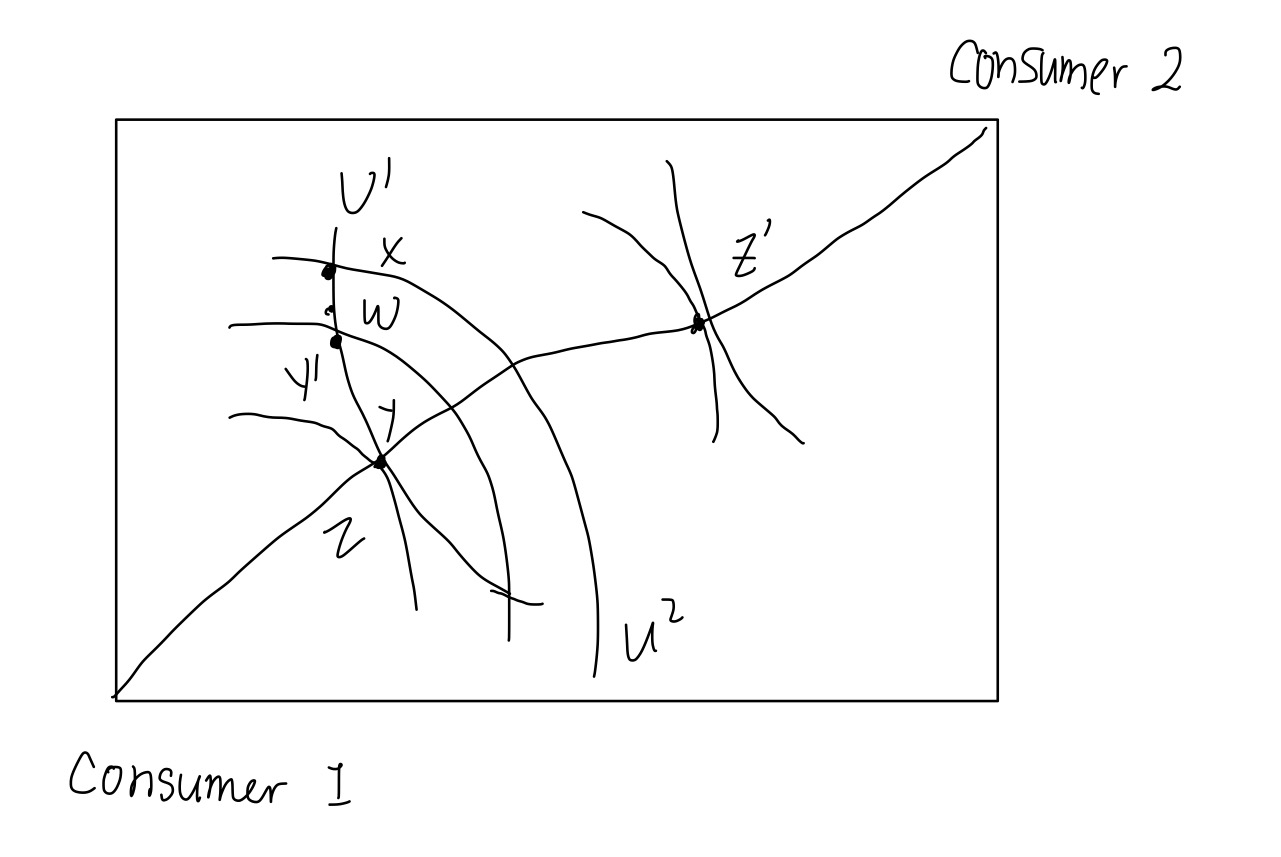
\includegraphics[scale = 0.2]{pareto-efficiency.jpg}\\
x is not P.E. because y leaves consumer 1 no worse off. but makes consumer 2 strictly better off. 
(Tangent point) Z is Pareto Efficiency. \\
(P.E. $\ne$ no worse than what consumer has but feasible set )\\
Origin is P.E. \\

Let $W(u^1,\dots, u^n)$ be a social welfare function that is strictly increasing in $u^i$\\
Ex. $ w = \alpha_1 u^1 + \alpha_2 u^2\dots +\alpha_n u^n,\, \sum a_i = 1, \alpha_i>0$\\
Ex. $ w = \frac{1}{n}\sum u^i \leftarrow$ Utilitarian social welfare\\
Ex. $ w = min\,\{u^1,\dots, u^n\} \leftarrow$ Rawlsian Welfare\\

Consider 
\begin{align*}
max\limits_x \, &W(u^1(x_1), \dots, u^n(x_n))\\
s.to \quad &x\in F(w)
\end{align*}
\underline{Result}: If $\bar{x}$ maximizes w, then $\bar{x}$ is P.E. \\
Proof: Suppose $\bar{x}$ is not P.E. there must be some $y \in F(w)$ such that \\$u^i(y_i) \ge u^i(\bar{x}_i) \,\forall i$ \\and  $u^j(y_j) > u^j(\bar{x}_j)$ for some j.\\
Then W at y $>$ W at $\bar{x}$(Since w is strictly increasing)\\
which implies $\bar{x}$ can't be maximizing, a contradiction. \\

How about the converse?\\
If $\bar{x}$ is P.E., is there a w that $\bar{x}$ maximizes s.to feasibility?\\
Here we specialize in 
\[W = \sum\limis_{i=1} ^{n} \alpha_i u^i, \, \alpha _i >0\]
\underline{Result}: Let $\bar{x}$ be a P.E. allocation, with $\bar{x}_i >> 0$, for all i .(Since $\bar{x}_i $ is vector) \\
Also, let $u^i$ be continuous, strictly increasing and strictly concave.\\
Then, there are some weights $(\bar{\alpha}_1, \dots, \bar{\alpha}_n) $ such that $\bar{x}$ maximizes w s.to feasibility. \\
$u^i = x^{\beta}y^{1-\beta}$ (Cobb-Douglas $\rightarrow$ CES $\Rightarrow$ Strictly  quasi-concave +HD1 $\Rightarrow$ Strictly concave (Hessian matrix))

\underline{Example1}:
\begin{align*}
    u^1 &= (x_1^1)^{\frac{1}{2}}(x_1^2)^{\frac{1}{2}}\\
    u^2 &= (x_2^1)^{\frac{2}{3}}(x_2^2)^{\frac{1}{3}}\\
    w_1 &= (\frac{1}{4},\frac{1}{4}) \qquad w_2 = (\frac{3}{4},\frac{3}{4})
\end{align*}
Since both are strictly quasi-concave. P.E. occurs at tangency point.\\
$MRS_{2,1}^1 = MRS_{2,1}^2 \Rightarrow \frac{x_1^2}{x_1^1} =2 \frac{x_2^2}{x_2^1}$ 
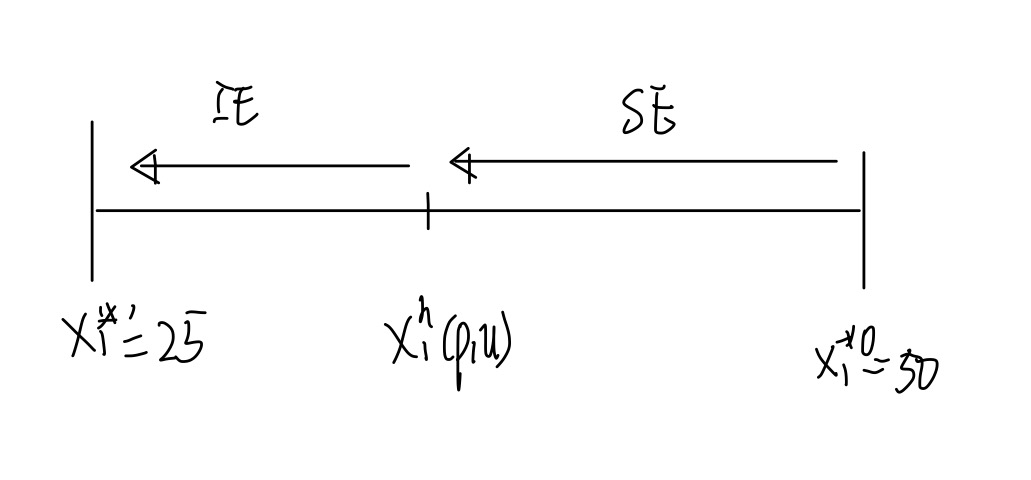
\includegraphics[scale = 0.15]{Example-1.jpg}
\\Feasibility \left\{
\begin{array}
x_1^1 + x_2^1 = \frac{1}{4} +\frac{3}{4} = 1\\
x_1^2 +x_2^2 = \frac{1}{4} +\frac{3}{4} = 1 \right\\
\end{array}

P.E. set $= \{ (x_1^1, x_1^2) \in [0,1]^2|x_1^2 = 2\frac{x_1^1}{1+x_1^1}\}$
\begin{align*}
max_x \, &w = \alpha u^1 +(1-\alpha)u^2\\
s.to \quad &x\in F(w)
\end{align*}
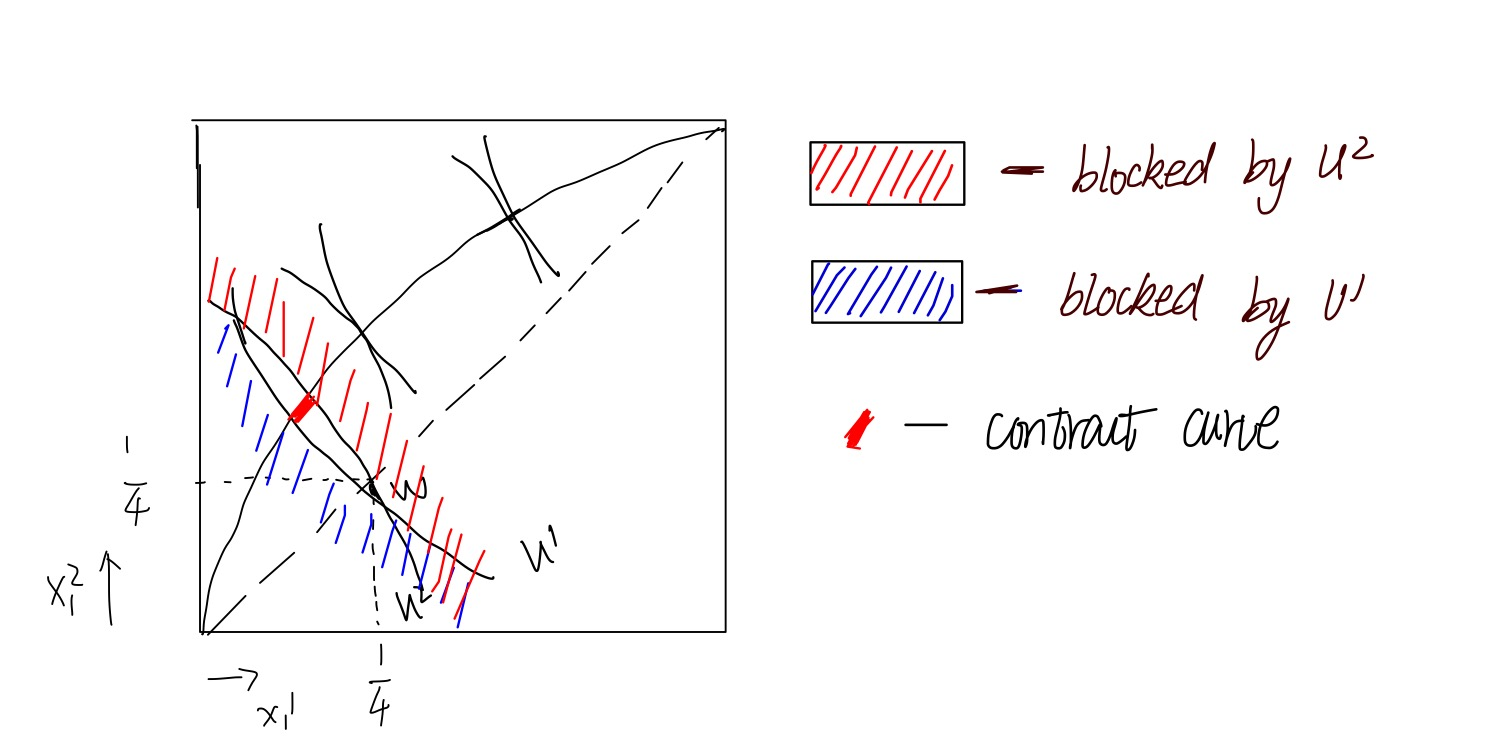
\includegraphics[scale = 0.25]{example1.jpg}\\
N=\{1,2\} \\
S= \{\{1\},\{2\},\{1,2\}\}\\
\underline{Definition} :Blocking Coalition\\
Let $S \subseteq N$ be a coalition of consumers. \\
We say that S blocks (improves on) $x \in F(w)$ if there is some allocation y such that
$ 1. \sum\limits_{i \in S} y_i \le \sum\limits_{i \in S} w_i$\\
(the allocation should be feasible)\\
$ 2. y_i \succeq_i x_i, \forall i\in S \text{ and }y_j \succ_j x_j \text{for some }j\in S$\\
(It should be Pareto Efficient)\\
\underline{Definition}: Core\\
A feasible allocation $x\in F(w)$ is in the core, $x_j \in C(w)$ if it canot be bloced by any coalition.\\
1) A special coalition: S=N-grand coalition\\
2) Another special coalition: S=\{i\}\\
Result: if x is in the core, it must be Pareto Efficient. \\
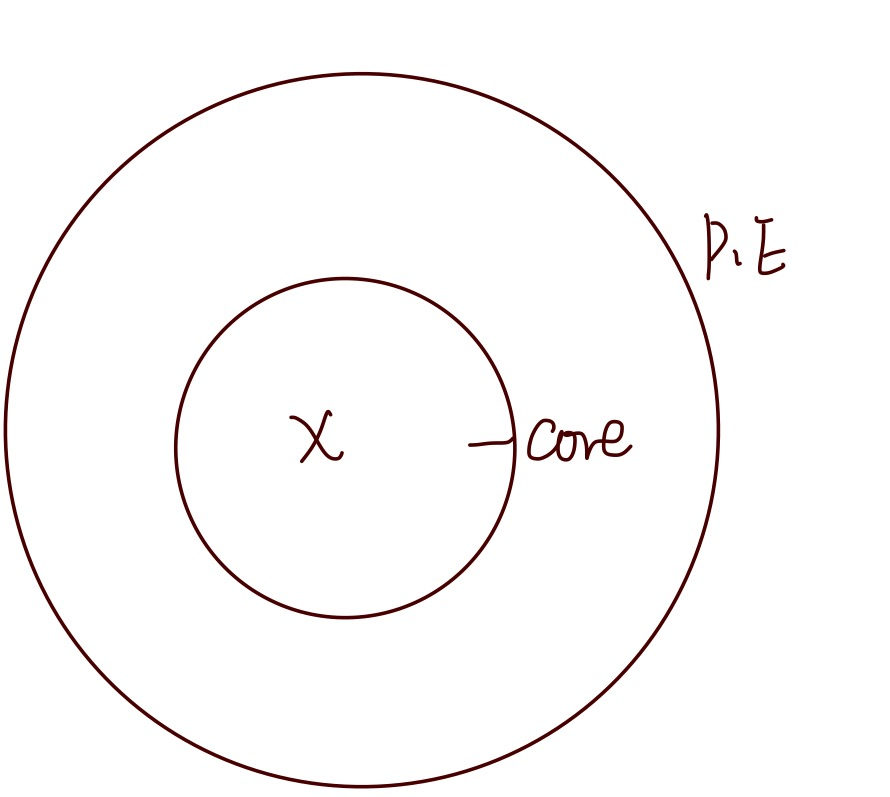
\includegraphics[scale = 0.1]{core.jpg}\\
Proof: 
Suppose x $\in$ C(w) but x is not P.E(S=N). \\
Then, there is another allocation y, $y_i \succeq_i x_i, \, \forall i$ but $y_j \succ x_j$, for some j\\
$\Rightarrow$ S=N blocks x $\Rightarrow$ not in the C(w) $\Rightarrow$ A contradiction.\\

Is the core non-empty, given $2^n -1$ possible coalitions to deter?($n= |N|$)\\

\underline{Example 2}\\
$u^1 = min\{x_1^1,x_1^2\}$ CES $\varrho \rightarrow -\infty$\\
$u^2 = max\{x_2^1,x_2^2\}$ CES $\varrho \rightarrow +\infty$\\
$w_1 = (\frac{1}{4}, \frac{1}{4}), w_2= (\frac{3}{4},\frac{3}{4})$\\
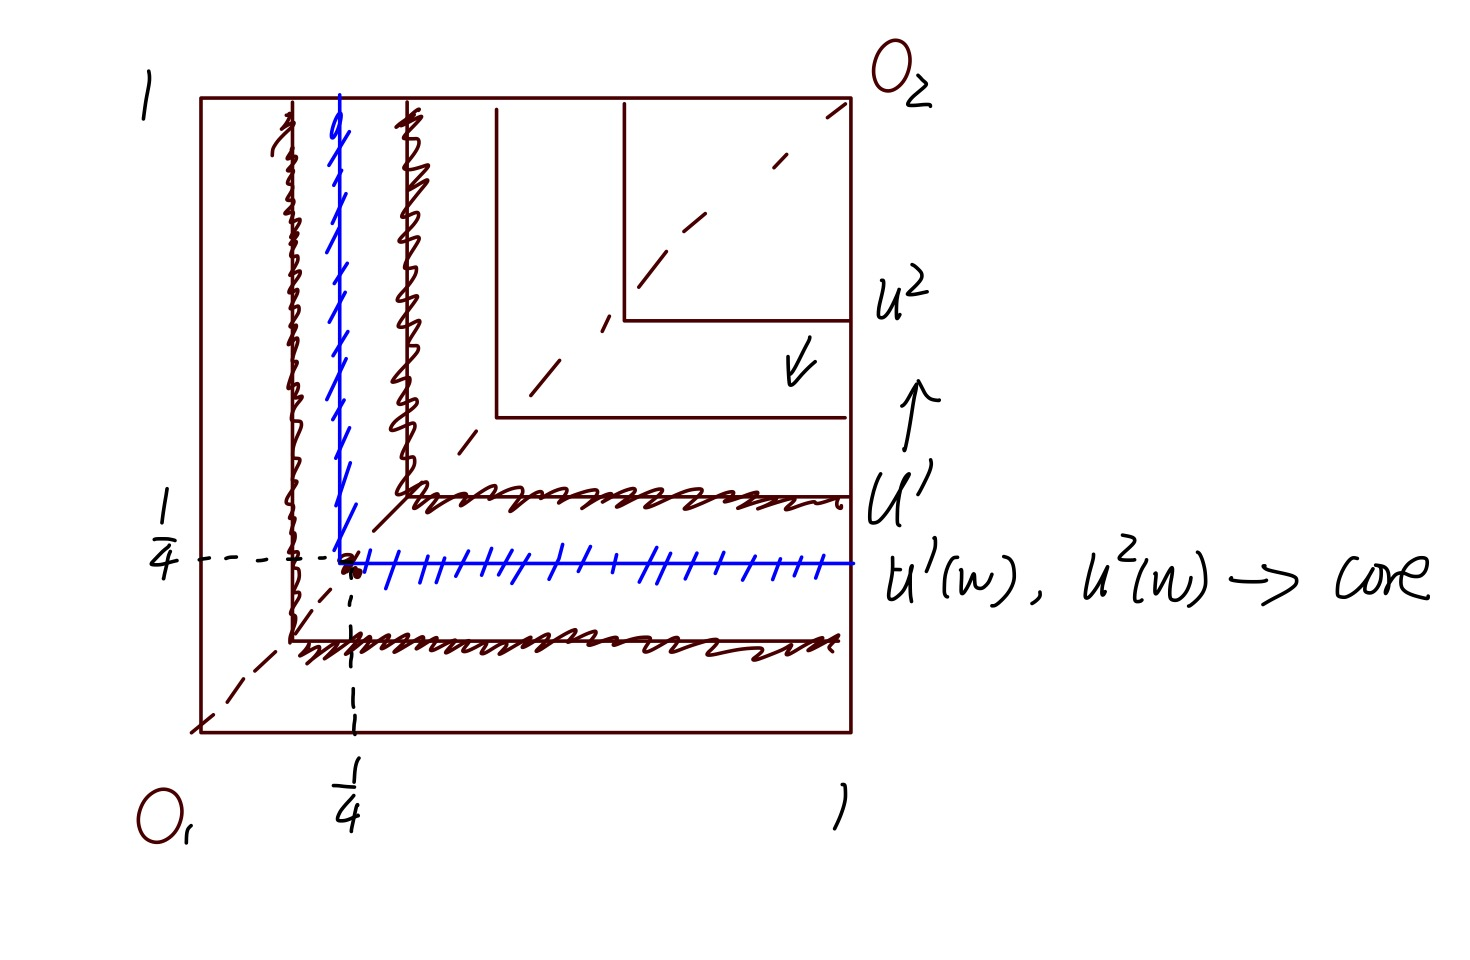
\includegraphics[scale = 0.2]{ezample2.jpg}\\
Aside: A CES u is strictly quasi-concave iff $\varrho < 1$\\
    \quad $ \,\quad u =(\sum \alpha_ix_i^\varrho)^{\frac{1}{\varrho}}, \sum\alhpa_i=1(\varrho = 1\rightarrow$ linear $\rightarrow$ quasi-concave)\\
    ($\varrho = 2, \rightarrow$ circle, $+\infty \rightarrow$ extreme of circle)\\
step:
\begin{enumerate}
    \item fix others' utility level and maximize one's utility
    \item repeat for each individual (find P.E)\\
        In example, P.E. is the whole box.
        \item utility should be at least better the initial endowment.  
        \begin{align*}
         u&(x_1) = u(w_1)  \\
         &\downarrow \qquad \downarrow\\
         (x_1^1, \dots, &x_1^k)\quad  (w_1^1,w_1^2,\dots,w_1k)
        \end{align*}
        Attention: Initial endowment can be in the core as eg.2.However, it can also be not in the core as eg.1.Then, utility is be higher than that in endowment but w not in the core. 
\end{enumerate} 
\subsection{Walrasian Equilibrium}
("Free market" equilibrium)\\

Assumption: Each consumer i has utility $u^i$, which is continuous, strictly increasing and strictly quasi-concave.\\
Consider a price vector $p = (p_1,\dots, p_k) >> 0$
\begin{align*}
    &market1 & &market2 & &market3\\
    &\msquare & &\msquare  & &\msquare\\
    &p_1\qquad & &p_2\qquad  & &p_3
\end{align*}
\begin{align*}
    max_{x_i}\quad &u^i(x_i) \\
    s.to\quad  &p\bullet x_i \le p\bullet w_i (\text{Income depends on price, in come is not longer fixed})\\
    &\Downarrow \qquad\quad  I_i\\
    x_i^* =& x_i^*(p,p\bullet w_i)\\
    &\qquad \quad I_i
\end{align*}
$x_i^*$ exists because $u^i$ is continuous (over a compact set)\\
$x_i^*$ is unique because $u^i$ is strictly q-concave.\\
$x_i^*$ is continuous in p because it is unique. \\

Result:\\
$x_i^*(p, p\bullet w_i)$ is unique. \\
Moreover, $x_i^*$ is continuous \underline{and} HD0 in p.\\
HDO: $x_i^*(tp,tp\bullet w_i) = x_i^*(p,p\bullet w_i),\forall t>0$\\
set $t = \frac{1}{p_1} > 0, \, tp=(\frac{p_1}{p_1},\frac{p_2}{p_1},\dots,\frac{p_k}{p_1}) = (1,\frac{p_2}{p_1},\dots,\frac{p_k}{p_1}) $(1st is numertaire)\\
set $t = \frac{1}{\sum p_i} > 0, \, tp=(\frac{p_1}{\sum p_i},\frac{p_2}{\sum p_i},\dots,\frac{p_k}{\sum p_i}) $\\
let $\hat{p}_j = \frac{p_j}{\sum p_i}, \sum \hat{p}_j = 1$\\

\underline{Definition} Excess Demand
\[Z^j(p) = \sum\limits_{i\in N} x_i^j(p,p\bullet w_i) - \sum\limits_{i\in N} w_i^j\]
\begin{center}
    Total demand for good j under prices p\\
    for every p, x is unique (according to the property above)
\end{center}
Excess demand vector: \\
$z(p) = (z^1(p), z^2(p),\dots,z^k(p))$\\
\underline{Note}: Excess supply: $z^j(p) < 0$ for some p \\
$\bullet$ Properties of z(p)
\begin{enumerate}
    \item z(p) is continuous in p (price vector)
    \item z(p) is HK0 in p
    \item Walras' law: $p\bullet z(p)=\sum\limits_{j=1}^{k} p_j z^j(p) = 0, \forall p>>0$\\
    \underline{Proof of (3)}
    \begin{align*}
        p\bullet z(p) &= \sum\limits_{j=1}^{k}p_jz^j(p)\\
        &= \sum\limits_{j=1}^{k}p_j(\sum\limits_{i\in N} x_i ^j(p,p\bullet w_i) - \sum\limits_{i \in N}w_i^j) \text{ (Full summation change order)}\\
        &= \sum\limits_{i \in N} \sum\limits_{j=1}^{k}p_j(x_i^j(.) - w_i^j)\\
        &= \sum\limits_{i \in N}(p\bullet x_i-p\bullet w_i) \\
        &= 0 \qquad \text{ = 0 (since $u^i$ is strictly increasing, budget binds)}
    \end{align*}
    Special cases: \\
        1) k=2, if $z^1(p)>0, z^2(p) < 0$\\
            \hspace*{6mm} Walras' law: $p_1 z^1(p) + p_2z^2(p) +\dots +p_kz^k(p) = 0$\\
        2) If $z^j(p) = 0$, for all $j \ne k$, then $z^k(p) = 0$\\
\end{enumerate}

\underline{Definition}: Walrasian Equilibrium (Free market)\\
\hspace*{6mm}A price vector $p^* \in R^k_{++}$ is said to be a Walrasian equlibrium if $z(p^*) = 0, \forall j = 1,2,\dots, k$\\
\hspace*{6mm}(Problem: with k equations, solution can still be a question e.g. $x^2 +1 = 0, x=  \mp i $)\\
\underline{Walrasian Allocations}: $x_i(p^*, p^*\bullet w_i$)\\
\underline{Theorem}: There exists a W.E.\\
\underline{Proof}(Arrow-Debreu, Mckenzie):\\
Define the following mapping:
\[ g^j(p) = \frac{p_j+max\{0,z^j(p)\}}{1+\sum\limits_{j=1}^{k}max\{0,z^j(p)\}}\text{(price adjustment)}\]
\[g(p) = (g^1(p),\dots, g^k(p))\]
\fbox{%
\begin{minipage}{6 in}

\\Aside: Brouwers' Fixed Theorem:\\
\hspace*{6mm}Any contious f mapping a non-empty, convex and compact (bounded and closed) set to itself, has a fixed point $f(x_0) = x_0\,\,(f(f(x_0)= f(x_0) = x_0)$.\\
Example: $f:[0,1]\rightarrow[0,1]\quad f(x) = x$\\
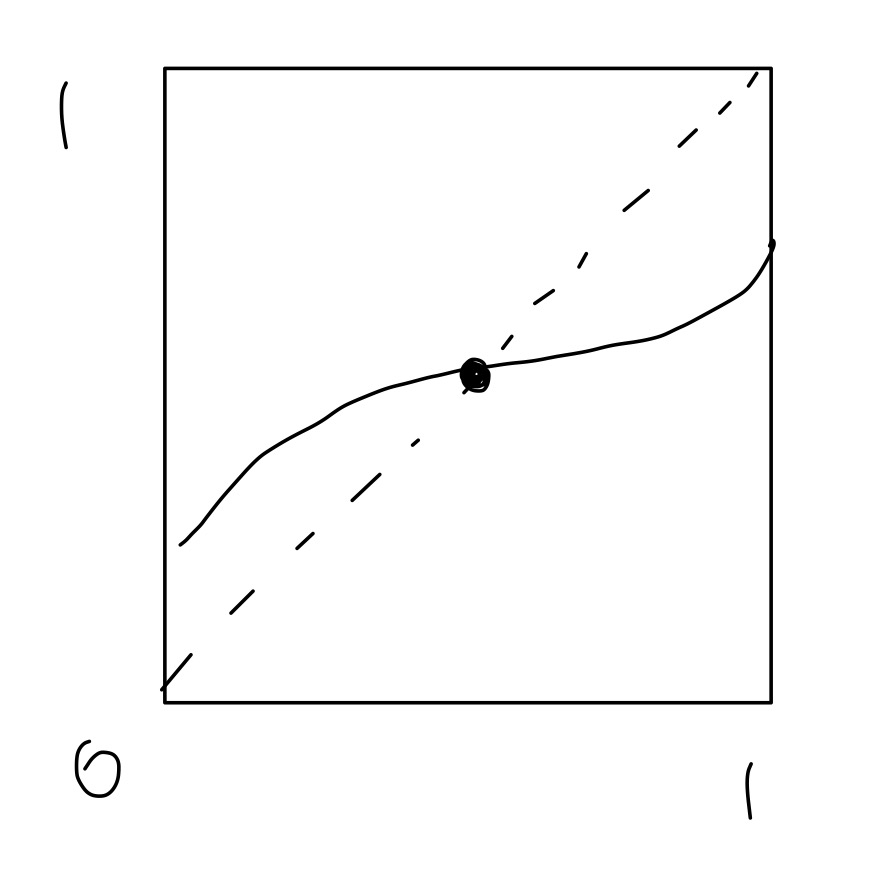
\includegraphics[scale = 0.15]{brouwer-1.jpg}\\The function f should pass through one point on f(x) =x
\end{minipage}
}

Normalize prices such that $\sum\limits_{j=1}^{k} p_j= 1$\\
\fbox{%
\begin{minipage}{6 in}
Aside: 
\[S = \{(y_1,\dots,y_n)|\sum\limits_i y_i =1, y_i\ge 0\}\]
$n=2, y_1+y_2 = 1\qquad n=3, y_1+y_2+y_3 =1$\\
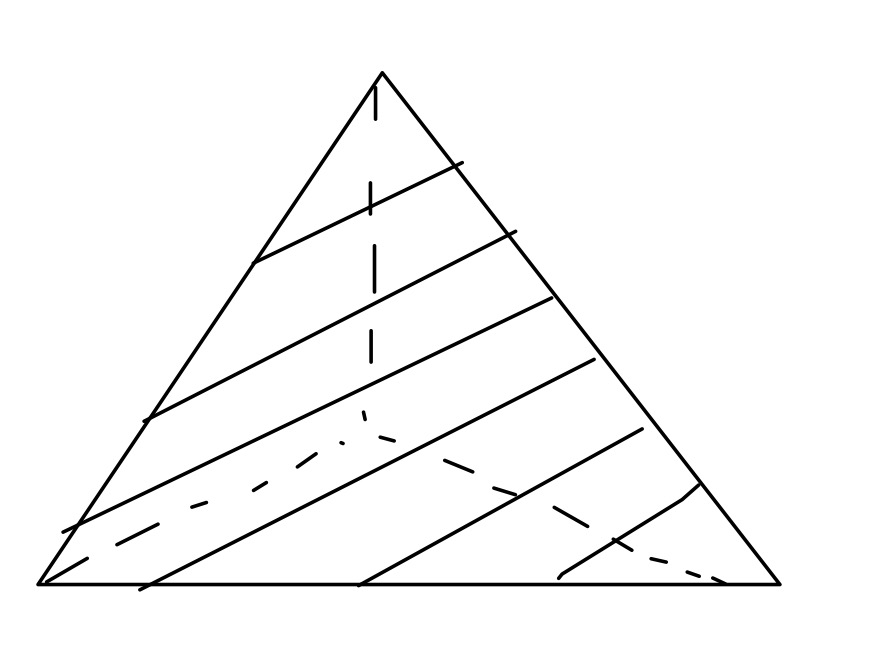
\includegraphics[scale = 0.1]{brouwer-2.jpg}\\
S is clalled simplex (non-empty, convex, bounded and closed.)
\end{minipage}}\\
Note that $\sum\limits_{j=1}^{k} =1$\\
Therefore, $g: S\rightarrow S$\\
By Brouver's Fixed pt Theorem\\
There is $p^* \in S$ such that $g(p^*) = p^*$\\
i.e. $g^j(p^*) = p_j^*$
\begin{align*}
p^*_j = \frac{p_j^*+max\{0,z^j(p^*)\}}{1+\sum\limits_{j=1}^{k}max\{0,z^j(p^*)\}} \\
    p_j^* + p_j^* \sum\limits_{j=1}^{k}max\{0,z^j(p^*)\} &= p_j^* +\,max\{0,z^j(p^*)\}\\
    \Rightarrow p_j^*\sum\limits_{j=1}^{k}max\{0,z^j(p^*)\} &=\,max\{0,z^j(p^*)\}\\
    \text{WTS: } z^j(p^*) &= 0, \forall j.\\
    \text{Multiple both sides by } & z^j(p^*)\\
    p_j^*z^j(p^*) \sum\limits_{j}max\{0,z^j(p^*)\} &= z^j(p^*) \,max\{0,z^j(p^*)\}\\
    \sum\limits_j( p_j^*z^j(p^*) )(\sum\limits_{j}max\{0,z^j(p^*)\})&= \sum\limits_j(z^j(p^*) \,max\{0,z^j(p^*)\})\\
   0 \quad \text{By walra's law} \quad \qquad &\\
   0 =\sum\limits_j(z^j(p^*)&\,max\{0,z^j(p^*)\})\\
   \text{Suppose } z^j(p^*)&> 0, \text{for some j}\\
   \text{Then, R.H.S}&= \ge 0+\ge 0+ \dots +> 0(j) +\ge 0+\dots\\
   &>0\\
   &\ne 0\\
   \text{Therefore, }z^j(p^*) &\le 0, \forall j\\
   \text{Suppose } z^j(p^*) &< 0, \text{for some j}
   \end{align*}
 \begin{align*}
    \text{Then, by walras' law}&\\
   p_1^*z^1(p^*) + p_2^*z^2(p^*)& +\dots+p_j^*z^j(p^*) +\dots+p_k^*z^k(p^*)  = 0\\
   \le 0\qquad \le 0\quad & \qquad \quad <0 \\
   \Rightarrow p_j^* &= 0 \text{  (Excess demand)}\\
   \Rightarrow z^j(p^*) &>0 \text{  (Since u is strictly increasing )}\\
   \rightarrow\leftarrow\\
   \text{Hence, } z^j(p^*) &= 0, \forall \,j
 \end{align*}
 \underline{Example}: Recall that  \begin{align*}
    u^1 &= (x_1^1)^{\frac{1}{2}}(x_1^2)^{\frac{1}{2}}\\
    u^2 &= (x_2^1)^{\frac{2}{3}}(x_2^2)^{\frac{1}{3}}\\
    w_1 &= (\frac{1}{4},\frac{1}{4}) \qquad w_2 = (\frac{3}{4},\frac{3}{4})
\end{align*}
 Since there are only two markets, we only need to clear one, say market 1. w.1.o.g. set $p_1=1$
\begin{align*}
     I_1 &= \frac{1}{4}1+\frac{3}{4}p_2 = \frac{1+p_2}{4} &
     I_2 &= \frac{3}{4}1+\frac{3}{4}p_2 = \frac{3(1+p_2)}{4}\\
     x_1^1&=\frac{\alpha I_1}{p_1} = \frac{p_2+1}{8} &x_2^1&=\frac{p_2+1}{2}\\
&\text{Market 1: }\text{Demand }= \text{Supply}&\\
&\frac{p_2+1}{8}+\frac{p_2+1}{2} = \frac{1}{4}+\frac{3}{4}\\
&\Rightarrow p_2^*= \frac{3}{5}
 \end{align*}
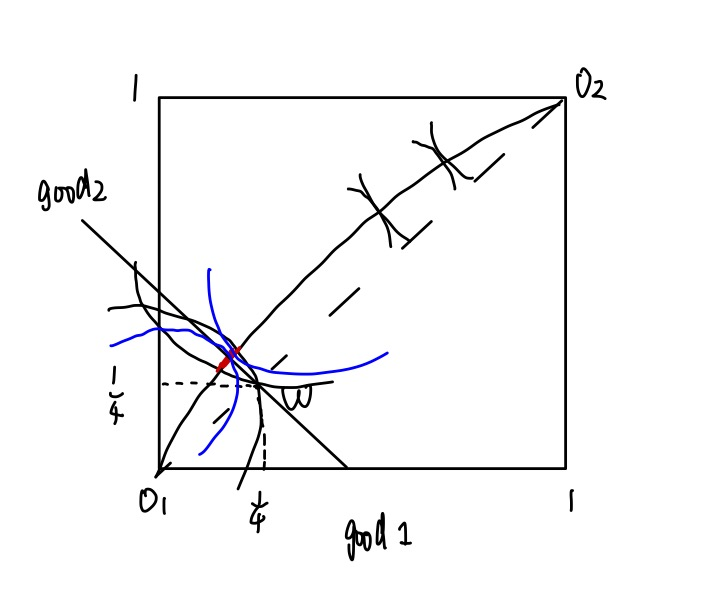
\includegraphics[scale = 0.2]{WEA-1.jpg}\\
Walrasian eq price: $p_1*^ =1, p_2^*=\frac{3}{5}(\frac{p_2^*}{p_1^*} = \frac{3}{5}$)\\
Walrasian eq allocations: $x_1^* = (\frac{1}{5},\frac{1}{3}$), $x_2^*=(\frac{4}{5},\frac{2}{3})$\\
Consumer 1: Net seller of good1, net buyer of good 2\\
P.E. considers only the grand coalition. S=N. (Like a unanity rule).\\
Core takes all coalitions into account. \\
S= \{\{1\},\{2\},\{1,2\}\}\\
(General equilibrium doesn't use price to allocate goods.\\
Walrasian equilibrium uses price to allocate goods. \\
\begin{rcases}
    max_{x_i}\quad u^i(x_i)\\
    s.to \quad p\bullet x_i \le p\bullet w_i\\
    \qquad \qquad I_i
\end{rcases}
$u^i(x_i^*)\ge u^i(w_i)$\\
$x_i = w_i$ is always feasible. \\
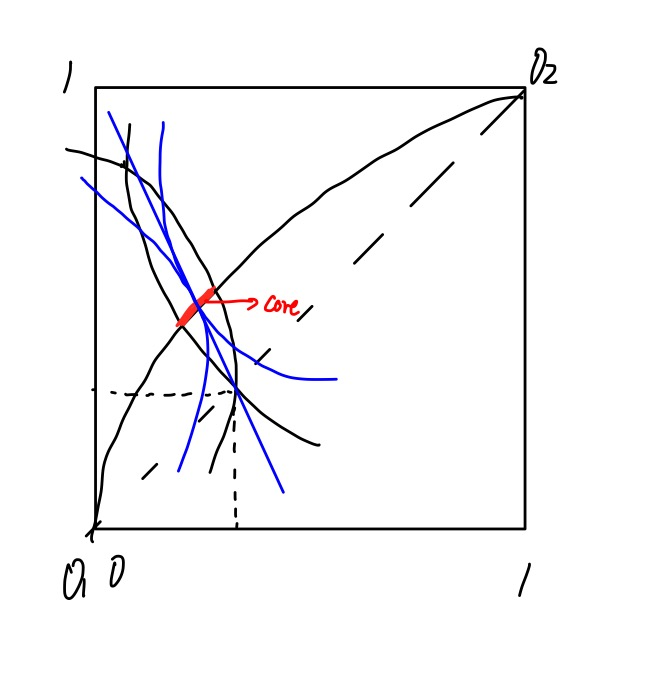
\includegraphics[scale = 0.2]{WEA-2.jpg}
\[MRS_{2,1}^1=\frac{p_1}{p_2} = MRS_{2,1}^2\]
\[\Rightarrow MRS_{2,1}^1 = MRS_{2,1}^2\]

(Core is pareto efficient $\Rightarrow$ Walrasian equilibrium must be P.E.  $\rightarrow$ First Welfare Theorem)\\
$\bullet$ Theorem: if $u^i$ is strictly increasing for all individual, then every Walrasian Equilibrium Allocation(WEA) is in the core.\\
(Don't assume quasi-concave because WEA is assumed to exist here. Then if no WEA, it doesn't affect the conditions)\\
\underline{Proof}:\\
Suppose not. That's suppose $x(p^*)$ is WEA (associated with a price vector p) but $x^(p^*)$ is not in the core. \\
Then, there's some coalition S that blocks $x(p^*)$.\\
In particular, there is some allocation $y\ne x(p^*)$ such that
\begin{enumerate}
    \item $\sum\limits_{i\in S} y_i \le \sum\limits_{i\in S} w_i$
    \item 
    $u^i(i_i)\ge u^i(x(p^*)), \forall i \in S $\\
    $u^j(y_j) > u^j(x(p^*)) \exists j \in S$
\end{enumerate}
    (But if $x(p^*)$ is W.E., y should be not feasible at least for some people)\\
    since $p^* \in R^k_{++}$ (1) $\Rightarrow \, p^* \sum\limits_{i\in S}y_i \le p^* \sum\limits_{i\in S}w_i $\\
    $\Rightarrow(2) p^*y \bullet y_i \ge p^* \bullet x_i(p^*) = p^* \bullet w_i \quad \forall i \in S\\
    p^*\bullet y_j > p^*\bullet x_j(p^*) = p^*\bullet w_j$\\
    Since $u^i$ is strictly increasing, budget binding. \\
    $p^*\sum\limits_{i\in S}y_i >p^* \sum\limits_{i\in S} w_i$\\
    Contradicting. $p^* \sum\limits_{i\in S}y_i \le p^* \sum\limits_{i\in S} w_i $\\
    Hence, $x(p^*)$ is in the core.\\

Implications:
\begin{enumerate}
    \item Since WEA are in the core.\\
    If there is a WEA, then core is nonempty. 
    \item since core $\Rightarrow $ Pareto Efficiency, Then WEAs are Pareto efficiency. \\
    \textbf{First Welfare Theorem}:\\
    If $u^i$ is strictly increasing for all, then any WEA is Pareto efficient.\\
    (S=N, Then proof above is for the theorem)\\
    (2nd welfare theorem $\Rightarrow$ pareto efficient is WEA if redistributing correctly)\\
\end{enumerate}
    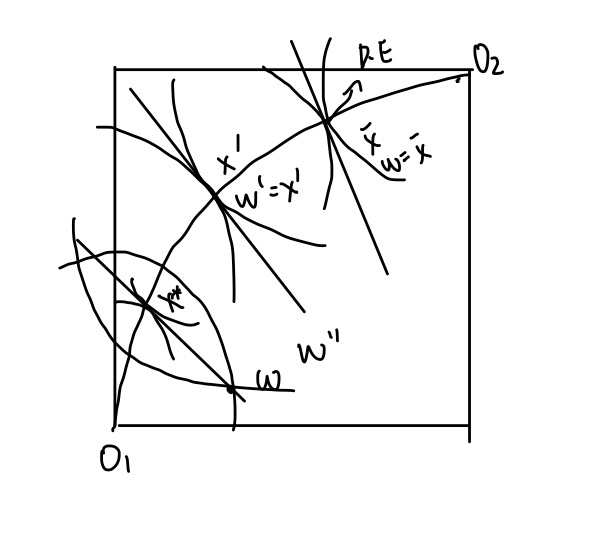
\includegraphics[scale = 0.3]{WEA-3.jpg}
\begin{enumerate}
    \item $x'$(External redistribution directly from w) is also a equilibrium.\\
    $\frac{p_1}{p_2} = MRS_{2,1}^1(X_1^-)$
    \item $w''$ (Move w to $w''$). The WEA $\Rightarrow$ x' automatically.\\
\end{enumerate}
    
$\bullet$ \textbf{Second Welfare Theorem}\\
Suppose $u^i$ is continuous, strictly increasing and strictly quasi-concave.\\
If $\bar{x}$ is Pareto Efficient, then there is some redistribution of w such that $\bar{x}$ is a WEA. \\
\underline{Proof}:\\
Suppose $\bar{x}$ is P.E. \\
Then it is feasible, $\bar{x} \in F(w)$\\
set $\hat{x} = \bar{x}$ (Make this P.E. the new w)\\
Given the assumption on $u^i$, there is a WEA $\hat{x}$, associated with $\hat{w}$.\\
WTS: $\hat{x} = \bar{x}$\\
Since $\hat{x}$ is WEA. 
\[U^i(\hat{x}_i) \ge U^i(\hat{w}_i)\, (=U^i(\bar{x}_i))\]
Suppose $U^j(\hat{x}_j) > U^j(\bar{x}_j)\quad \exists j \in N$\\
But then $\hat{x}$ can't be P.E. A contradiction. \\
$u^i(\hat{x}_i) = u^i(\bar{x}_i)\quad \forall i\in N$\\

Suppose $\hat{x}_j \ne \bar{x}_j$.\\
Then, there is some $\hat{\hat{x}}$ that's feasible for j but by strictly quasi-concavity, $u^j(\hat{\hat{x}})> u^j(\hat{x)}$\\
Contradicting $\hat{x_j}$ being utility maximizing. \\
Hence, $\hat{x}_j = \bar{x}_j, \forall j$\\
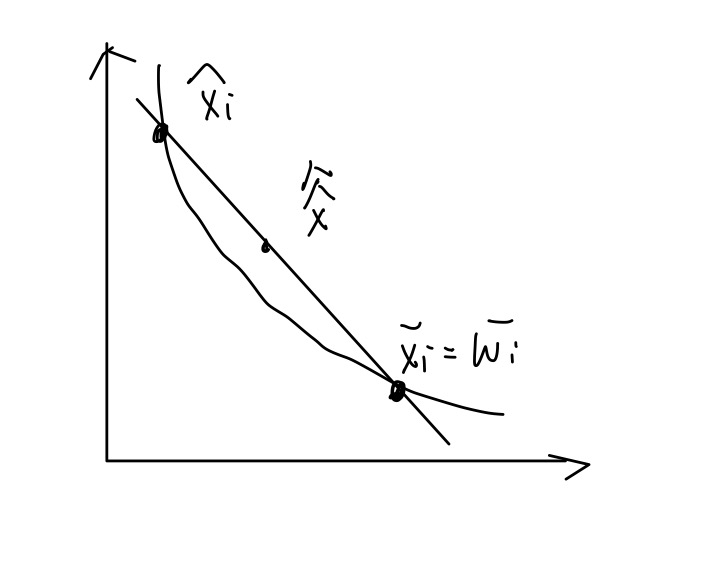
\includegraphics[scale = 0.2]{WEA-4.jpg}\\
\underline{Example}\\
Recall that 
\[MRS_{2,1}^1 = \frac{x_1^2}{x_1^1}\]
P.E. set \[x_1^2 = \frac{2x_1^1}{1+x_1^1}\]
Let $x_1^1 = \frac{1}{2} \Rightarrow x_1^2 = \frac{2}{3}$\\
$\bar{x}_1= (\frac{1}{2},\frac{2}{3})\quad \bar{x}_2 = (\frac{1}{2}, \frac{1}{3})$ P.E.\\ $w' = \bar{x}$\\
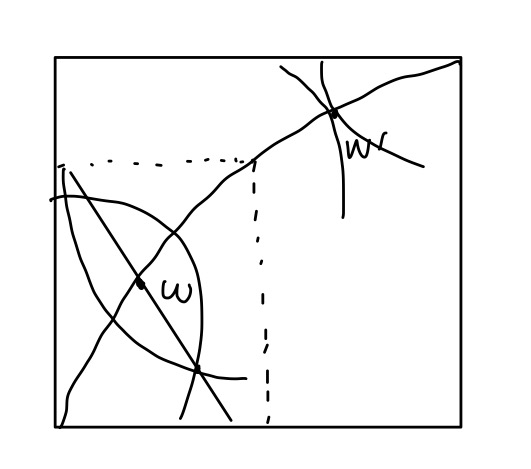
\includegraphics[scale = 0.3]{WEA-5.jpg}\\
Q: give us all initial endowment possibilities that engender $\bar{x}$ as a WEA. (As long as w on $\frac{p_1}{p_2}$ line $\rightarrow$ WEA $\bar{x}$)\\
$MRS_{2,1}^1 = \frac{4}{3}$\\
Set $\frac{p_1}{p_2} = \frac{4}{3}.$ \\
Let $p_1^* = 1, \, p_2^* = \frac{3}{4}$\\
$p_1^* \bar{x}_1^* + p_2^*\bar{x}_1^2 = p_1^*w_1^1 +p_@^*w_1^2$\\
$\Rightarrow w_1^1 + \frac{3}{4}w_1^2 = 1 \qquad w_1^1 + w_2^1 = 1$\\
$w_2^1 +\frac{3}{4}w_2^2 =\frac{3}{4}\qquad w_1^1 +w_2^2 =1 $\\

$max_{x_i} \qquad u^i(x_i)$\\
s.to $\quad p\bullet x_i \le p \bullet w_i$ (P is given, small buyer)\\
Types A   B\\
      $u^A \quad u^B$\\
      $u^A \quad u^B$\\
      $x= (x_A,x_B)$\\
Two-fold economy\\
    A,A,B,B
    $x = (x_{A1},x_{A2}, x_{B1}, x_{B2}) \Rightarrow$ no, of allocation in core changes.\\

r-fold economy\\
$t = \{ 1,\dots, I\}$ - types of consumers (with some utility \underline{AND} initial endowment)\\
$\varepsilon_r = $ r-fold economy with r type t consumers. \\

$\bullet$ Theorem: Equal treatment in the core\\
Suppose $u^i$ is continuous, strictly increasing and strictly quasi-concave. \\
If x is in the core of $\varepsilon_r$, then every t-type consumer must have the same bundle.
\[x_{ti} = x_{tj}\]

\underline{Proof}\\
For simplicity, let $t = A, B, r=2$. Then, $x= (x_{A1},x_{A2},x_{B1}, x_{B2})$\\
Suppose $x\in C_2$, but $x_{A1} \ne x_{A2}$, WLOG. 
\[u^A(x_{A1} )\ge u^A(x_{A2})\]
\[\text{and }u^A(x_{B1} )\ge u^A(x_{B2})\]
Consider the worse-off consumer $A2$ and $B2$, and assign this allocation
\[\bar{x}_{A2} = \frac{x_{A1}+x_{A2}}{2}, \bar{x}_{B2} = \frac{x_{B1}+x_{B2}}{2}\]
Since $x_{A1} \ne x_{A2}$ and $u^A$ is strictly quasi-concave. 
\[u^A(\bar{x}_{A2})> u^A(x_{A2}) \text{. Moreover, }\]
\[u^B(\bar{x}_{B2})\ge u^B(x_{B2}) \text{(We don't assume $x_{B2} \ne x_{B1}\Rightarrow$ x not $>$)} \]
Need to check feasibility of $\bar{x}_{A2} $ and $\bar{x}_{B2}$ for $S = \{A2, B2\}.$\\
$\bar{x}_{A2} + \bar{x}_{B2} \le (?) w_A + w_B$\\
$\frac{x_{A1}+x_{A2}+x_{B1}+x_{B2}}{2}\le \frac{2w_A + 2w_B}{2} = w_A + w_B$\\
Because $x\in C_r$ and this X is P.E. $\Rightarrow$ possible in the entire economy. \\

Hence, $(\bar{x}_{A2},\bar{x}_{B2})$ is feasible for $S=\{A_2, B_2\}$\\
Then, S blocks x, contradicting $x \in C_r$\\
Hence, $x_{A1} = x_{A2}$, and  $x_{B1} = x_{B2}$.\\

By the equal treatment property, 
\[C_r = \{x\in F(w)| x_1, \dots, x_1, x_2,\dots, x_2,\dots, x_I,\dots,x_I\}\]
\[\qquad \qquad \qquad \text{r times} \qquad \text{r times} \qquad \text{r times}\]

To compare $C_r$ and $C_{r^'}$, focus on $(x_1,\dots, x_I) $ (One represent the type)\\
\underline{Result}:Shrinking core.
\[C_1\supseteq C_2\supseteq \dots \supseteq C_r \supseteq\]
\underline{Proof}:\\
Suppose $x=(x_1,\dots,x_n) \in C_r $ but $x \not\in C_{r-1}$\\  
Then there is some S of $\varepsilon_{r-1}$ that blocks x but S is also feasible under $\varepsilon_r$ and would again block x in $\varepsilon_r$. A contradiction, $x\in C_r$.\\

The core shrinks but wiil it disappears?\\
$\bullet$ Theorem: Edgeworth-Debreu-Scarf\\
$u^i$ is continuous, strictly increasing and strictly quasi-concave. \\
If $x\in C_r$ ,for every $r= 1,2,\dots, n$\\
then x is a WEA in the orginal economy $\varepsilon_1$.

Recall WEA in the example. \\
$x_1^* = (\frac{1}{5}, \frac{1}{3})$\\
$x_2^* = (\frac{4}{5},\frac{1}{3})$\\

Proof:\\
Consider 2 types of consumer A and B. \\
Suppose $\tilde{x} \in C_r$, for all r but $\tilde{x}$ is not a WEA in $\varepsilon_1$. \\
Then $\tilde{x} \in C_r$ and P.E. in $\varepsilon_r$, specially $MRS_{2,1}^A (\tilde{x}_A) = MRS_{2,1}^B(\tilde{B})$(Since u is strictly quasi-concave.\\
Since $\tilde{x} $ is not WEA in $\varepsilon_1$, either $\frac{p_1}{p_2} \ne MRS_{2,1}^A (\tilde{x}_A) $ or $\frac{p_1}{p_2} \ne MRS_{2,1}^B(\tilde{x}_B).\\

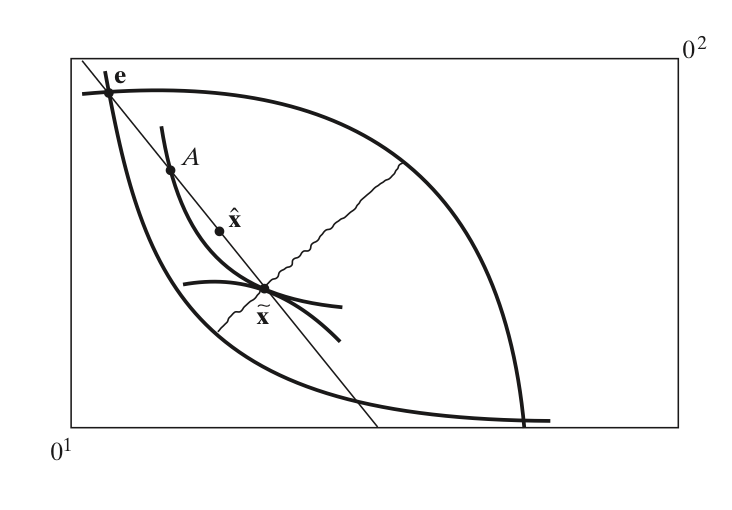
\includegraphics[scale = 0.5]{edgeworth-debreu-scarf.png}\\
WLOG, suppose $\frac{p_1}{p_2} \ge MRS_{2,1}^A (\tilde{x}_A) $\\
Then there is some $\hat{x}$ such that 
\[\hat{x}_A = \frac{1}{r}w_A + \frac{r-1}{r}\tilde{x}_A\]
\[t \qquad 1-t\]
Consider the coalition S= r type A + (r-1) type B is an r-fold economy\\
Given $\hat{x}$ to type A's, $\tilde{B}$ to type B's. \\
Clearly $u^A(\hat{x}_A) >u^A(\tilde{x}_A)$ (By strict quasi-concavity\\
and $u^B(\tilde{B}) = u^B(\tilde{B})$\\
Feasibility?\\
$r\hat{x}_A +(r-1) \tilde{x}_B \le rw_A + (r-1) w_B$
\begin{align*}
   r[\frac{1}{r}w_A + \frac{r-1}{r}\tilde{x}_A ]+ (r-1) \tilde{x}_B &= w_A + (r-1) (\tilde{x}_A +\tilde{x}_B) \\
   &\le w_A +(r-1) (w_A +w_B) \\
   &= rw_A + (r-1)w_B
\end{align*}
So, $\hat{x}_B$ and $\tilde{x}_B$ are feasible in S and do better, \\
contradicting $\tilde{x}$ being in $C_r$.\\
Hence, 
\begin{align*}
    \frac{p_1}{p_2} &= MRS_{2,1}^A(\tilde{x}_A)\\
    &=MRS_{2,1}^B(\tilde{x}_B)
\end{align*}\includegraphics[scale = 0.2]{graph/wea.jpg}\\
\underline{Example}: \\
WE prices: $p_1^* = 1, p_2^* = \frac{3}{5}$\\
WEA $x_1^* = (\frac{1}{5}, \frac{1}{3}), x_2^* = (\frac{4}{5}, \frac{2}{3})$,(given price, only one WEA ).\\
\includegraphics[scale = 0.15]{graph/weapecore.jpg}\\
When n increases to infinity, WEA approaches core (WEA is the only left). Correspond to that in large economy, price-taking assumption. \\
Price mechanism allocate goods. Only need to know one's own utility function, initial endowment, and price vector to get the WEA , then can get core(No need to know everyone's utility func to get core). 
However, WE might not be unique. It can have multiple results. \\

The uniqueness of Walrasian eq. \\
We don't need be unique. \\
Example: 
\begin{align*}
    u^1 &= x_1^1 -\frac{1}{8}(x_1^2)^{-8}\\ 
    u^2 &= -\frac{1}{8}(x_2^1)^{-8} + x_2^2\\
    w_1 &= (2,r) , w_2 = (r,2), r= 2^{\frac{8}{9}}  - 2^{\frac{1}{9}}\\
    x_1^1 &= 2 + r \frac{p_2}{p_1} -(\frac{p_2}{p_1})^\frac{8}{9}\\
    x_2^1 &= (\frac{p_1}{p_2})^{-\frac{1}{9}}\\
    \text{set } p_2 &=1, p_1 = p\\
    z^1(p) &= r(\frac{1}{p} - 1) - (\frac{1}{p})^{\frac{8}{9}} +(\frac{1}{p})^{\frac{1}{9}}\\
    z^1(p) &= x_1^1 +x_2^1 -(w_1^1 +w_2^1)
\end{align*}
\includegraphics[scale = 0.25]{graph/nonuniquewea.jpg} \\
Three WE prices. $(p_1, p_2) = (\frac{1}{2},1) = (1,1)= (2,1)$\\

\underline{Definition}: Gross substitute\\
Two goods , i and j,are gross substitutes if $\frac{\partial z^j(p)}{\partial p_i} > 0$, for $i \ne j$\\
Theorem: suppose all goods are gross substitutes, then $p^* $ is a WE price vector, then it is unique (up to multiples). \\
\underline{Proof}:\\
suppose $p' \ne p^*$ is another equilibrium price vector. \\
$p' = (p'_1, \dots, p'_n), p^*= (p_1^*,\dots, p_n^*)$\\
Consider $\frac{p_1'}{p_1^*},\frac{p_2'}{p_2^*},\dots,\frac{p_k'}{p_k^*},\dots,\frac{p_n'}{p_n^*}$\\
Let $\frac{p_k'}{p_k^*}$ be the highest and call $\frac{p_1'}{p_1^*} = m, \Rightarrow p_k' = ,p_k^*$\\
$\frac{p_1'}{p_1^*} \le m \Rightarrow p_1'\le mp_1^*$\\
Consider $z^k(mp^*) = 0$, (because $z^k(p^*) = 0 $& z(p) is HDO)\\
\[z^k(mp_1^*, \dots, mp_k^*,\dots, mp_n^*) = 0\]
\[ \downarrow \qquad \downarrow \qquad \downarrow\]
\[ p_1' \qquad p_k' \qquad p_n'\]
$\Rightarrow $ (gross substitute) $z^k(p') < 0 \Rightarrow z^k(p') \ne 0$, contradicting $p'$ being a W.E. \\
Then, $p' = p^*$  (Allocation is unique)\\

$\frac{p_1^*}{p_2^*}$ not unique $\Rightarrow$ unique $x^* x_i^*(p_i^*, p_{-i}^*,w_i)$\\
True if $x_i(p,p\bullet w_i)$ is a function of p. 
\begin{align*}
    max_{x_i} \quad &u^i \\
    s.to \quad &p\bullet x\le I\\
    &\Downarrow\\
    &x_i^*\text{if $u^i$ is continuous in $x_i$, is unique if $u^i$ is strictly quasi-concave}
\end{align*}

\end{document}
